\documentclass[twoside,11pt]{article}

\usepackage{jmlr2e} % must come before other packages
\usepackage{amsmath,amssymb,bm,booktabs,array,microtype}
\usepackage[section]{placeins}
\usepackage{siunitx}
\sisetup{group-separator={,}}
\usepackage[ruled,vlined]{algorithm2e}
\DontPrintSemicolon

\graphicspath{{../figures/revision/}{../figures/full/}{../figures/mimic_local/}}

\newcommand{\A}{\mathcal A}
\newcommand{\E}{\mathcal E}
\newcommand{\Pp}{\mathbb P}
\newcommand{\Ee}{\mathbb E}
\newcommand{\R}{\mathbb R}
\newcommand{\dist}{\operatorname{dist}}
% Name of the proposed procedure; change it here only.
\newcommand{\method}{MiSCert}

\newcommand{\CalMultCoverage}{0.928}
\newcommand{\CalPointCoverage}{0.514}
\newcommand{\CalExactCoverage}{0.960}
\newcommand{\CalNormalCoverage}{0.938}
\newcommand{\CalMultContainment}{0.998}
\newcommand{\CalHoeffARR}{0.138}
\newcommand{\CalHolmARR}{0.270}
\newcommand{\MainMultARR}{0.297}
\newcommand{\MainExactARR}{0.258}
\newcommand{\RareMultCoverage}{0.780}
\newcommand{\RareExactCoverage}{0.995}
\newcommand{\LargeMultCoverage}{0.910}
\newcommand{\StressIdenticalReps}{200}
\newcommand{\StressReps}{200}
\newcommand{\NestedReps}{200}
\newcommand{\CalibrationReps}{500}
\newcommand{\ReferenceN}{20000}
\newcommand{\MissingnessReps}{100}
\newcommand{\PowerReps}{400}
\newcommand{\PowerCells}{48}
\newcommand{\PowerAnalyticMaxDev}{0.019}
\newcommand{\PowerMultCovMin}{0.610}
\newcommand{\PowerMultCovMax}{0.955}
\newcommand{\PowerMultCovMinSmallK}{0.810}
\newcommand{\PowerExactCovMin}{0.948}
\newcommand{\PowerMinContainment}{0.965}
\newcommand{\PowerHolmGainMax}{0.102}
\newcommand{\PowerMultGainMax}{0.337}
\newcommand{\PlanRatioMin}{0.34}
\newcommand{\PlanRatioMax}{0.40}
\newcommand{\PlanHoeffProbMin}{0.50}
\newcommand{\PlanHoeffProbMax}{0.53}
\newcommand{\PlanExactSmall}{422}
\newcommand{\PlanHoeffSmall}{1,243}
\newcommand{\PowerSmallN}{250}
\newcommand{\PowerLargeN}{8,000}
\newcommand{\PowerKsmall}{25}
\newcommand{\PowerKlarge}{100}
\newcommand{\PowerMultCovSmallKLo}{0.810}
\newcommand{\PowerMultCovSmallKHi}{0.853}
\newcommand{\PowerMultCovLargeKLo}{0.610}
\newcommand{\PowerMultCovLargeKHi}{0.733}
\newcommand{\PowerMultCovLargeNLo}{0.907}
\newcommand{\PowerMultCovLargeNHi}{0.955}
\newcommand{\PowerMultBestGainCov}{0.610}
\newcommand{\PlanExactDeltaFiveLo}{422}
\newcommand{\PlanExactDeltaFiveHi}{626}
\newcommand{\PlanExactDeltaOneLo}{12,179}
\newcommand{\PlanExactDeltaOneHi}{18,235}
\newcommand{\PlanExactProbAtHoeffMin}{0.999}
\newcommand{\AnatReps}{500}
\newcommand{\AnatMultReproduced}{466}
\newcommand{\AnatExactFailures}{20}
\newcommand{\AnatExactSafeOnly}{9}
\newcommand{\AnatExactFalseCert}{1}
\newcommand{\AnatMultFailures}{34}
\newcommand{\AnatMultSafeOnly}{19}
\newcommand{\AnatMultFalseCert}{1}
\newcommand{\AnatMultCoverageRerun}{0.932}
\newcommand{\StressContMultCrit}{2.87}
\newcommand{\StressContAgree}{200}
\newcommand{\StressRareMultCrit}{2.82}
\newcommand{\StressRareAgree}{199}
\newcommand{\StressBonfCrit}{2.88}
\newcommand{\StressRareLowCountShare}{61}
\newcommand{\GainExactMin}{0.016}
\newcommand{\GainExactMax}{0.092}
\newcommand{\TailLargeKSmallNLo}{8.6}
\newcommand{\TailLargeKSmallNHi}{9.6}
\newcommand{\TailLargeKLargeNLo}{1.5}
\newcommand{\TailLargeKLargeNHi}{1.6}
\newcommand{\TailSmallKLargeNLo}{1.3}
\newcommand{\TailSmallKLargeNHi}{1.3}
\newcommand{\TailLargeKHugeNLo}{1.2}
\newcommand{\TailLargeKHugeNHi}{1.2}
\newcommand{\BootDiffBLow}{200}
\newcommand{\BootDiffBHigh}{5,000}
\newcommand{\BootDiffSdLow}{0.123}
\newcommand{\BootDiffSdHigh}{0.021}
\newcommand{\BootSameCount}{72}
\newcommand{\OrigPython}{3.12.7}
\newcommand{\OrigNumpy}{1.26.4}
\newcommand{\RevPython}{3.14.3}
\newcommand{\RevNumpy}{2.5.4}
\newcommand{\RevScipy}{1.18.1}
\newcommand{\RevPandas}{3.0.6}
\newcommand{\RevSklearn}{1.9.1}
\newcommand{\BootSeeds}{25}
\newcommand{\ContExactFirstRecall}{0.343}
\newcommand{\ContMultFirstRecall}{0.379}
\newcommand{\ContExactFirstGrid}{6}
\newcommand{\ContExactFirstSafeGrid}{19}
\newcommand{\ContExactFirstUnsafe}{0}
\newcommand{\ContReps}{200}
\newcommand{\MimicEligible}{60}
\newcommand{\MimicConditions}{72}
\newcommand{\MimicMaxExactUpper}{0.047}
\newcommand{\MimicMaxHoeffUpper}{0.104}
\newcommand{\EssK}{72}
\newcommand{\EssZeroDeaths}{33}
\newcommand{\EssZeroFNUpperFourteen}{0.405}
\newcommand{\EssBestLowerFourteen}{0.595}
\newcommand{\EssSmallDeathsMin}{5}
\newcommand{\EssSmallDeathsMax}{14}
\newcommand{\EssLargeDeaths}{1,092}
\newcommand{\EssDeathsEightyFive}{995}
\newcommand{\EssDeathsNinety}{230}
\newcommand{\EssDeathsNinetyFive}{87}
\newcommand{\EssDeathsEightyFiveNinety}{1,205}
\newcommand{\WdbcExactFullLR}{0.160}
\newcommand{\WdbcExactFullET}{0.166}
\newcommand{\WdbcExactFullHGB}{0.233}
\newcommand{\WdbcExactFirstLR}{0.053}
\newcommand{\MimicAlwaysFull}{0.041}
\newcommand{\ProfileFnLargeMin}{0.185}
\newcommand{\ProfileFnLargeMax}{0.242}
\newcommand{\ProfileFnSmallMinUpper}{0.698}
\newcommand{\EssPrevLo}{0.6}
\newcommand{\EssPrevHi}{1.2}
\newcommand{\EssAdmissionsLo}{20,000}
\newcommand{\EssAdmissionsHi}{38,000}
\newcommand{\SensMultCovHighRho}{0.967}
\newcommand{\SensMultCovSmallN}{0.903}

% ================= Figure requirements =================
% Add these ONCE in the preamble of main.tex, before \begin{document}.
\usepackage[T1]{fontenc}
\usepackage{lmodern}
\usepackage{amsmath,amssymb}
\usepackage{xcolor}
\usepackage{graphicx} % for \resizebox
\usepackage{tikz}
\usepackage{pgfplots}
\usetikzlibrary{arrows.meta,positioning,calc,fit,backgrounds,shapes.geometric}
\pgfplotsset{compat=1.18}

% ---------- Palette ----------
\definecolor{navy}{HTML}{123E73}
\definecolor{blue}{HTML}{2F8BCB}
\definecolor{blueDark}{HTML}{1F6FAE}
\definecolor{blueBorder}{HTML}{7DB8E3}
\definecolor{blueLight}{HTML}{EEF7FD}
\definecolor{green}{HTML}{56B67A}
\definecolor{greenDark}{HTML}{2D8B55}
\definecolor{greenBorder}{HTML}{A2D8B5}
\definecolor{greenLight}{HTML}{EFF9F2}
\definecolor{grayText}{HTML}{4E6072}
\definecolor{yellow}{HTML}{F6D85B}
\definecolor{red}{HTML}{D9463E}
\definecolor{redLight}{HTML}{FBE9E8}
\definecolor{safeGreen}{HTML}{159447}

% ---------- TikZ styles ----------
\tikzset{
  topPanel/.style={rounded corners=2.5mm, line width=.7pt, inner sep=0pt},
  topHeader/.style={rounded corners=2.5mm, minimum height=1.25cm, text=white,
    font=\bfseries\fontsize{9.6}{11}\selectfont, align=center},
  body/.style={font=\fontsize{8.4}{10}\selectfont, align=center, text=navy},
  num/.style={circle, minimum size=7.2mm, inner sep=0pt, text=white,
    font=\bfseries\large, line width=.8pt, draw=white},
  flow/.style={-{Stealth[length=3.1mm,width=2.7mm]}, line width=1.5pt, blue},
  note/.style={rounded corners=2mm, align=center, inner sep=5pt,
    font=\fontsize{7.7}{9.1}\selectfont, text=navy},
}
% ===============================================================


\ShortHeadings{Statistical Assurance Regions}{Maale and Yi}
\firstpageno{1}

\begin{document}

\title{Statistical Assurance Regions for Predictive Models Under Joint Distribution Shift and Missingness}

\author{\name Faustus Domebale Maale \email fdmaale@aggies.ncat.edu \\
\addr Applied Science and Technology Ph.D. Program\\
College of Science and Technology\\
North Carolina A\&T State University, Greensboro, NC, USA
\AND
\name Hui Yi \email hyi@ncat.edu \\
\addr Department of Mathematics \& Statistics\\
North Carolina A\&T State University, Greensboro, NC, USA}

\editor{}
\maketitle

\begin{abstract}%
Deployment changes in populations and measurement availability can undermine
predictive performance, making test-set averages insufficient for identifying
conditions that meet a specified risk tolerance. We define statistical
assurance regions (SARs) over prespecified environments jointly modeling
missingness and distribution shift, with risk defined as expected bounded
loss. We estimate conservative inner SARs contained in the true
region with probability at least $1-\alpha$: in finite samples using
exact-binomial and bounded-loss procedures, and asymptotically using an
optional Gaussian multiplier band. Simulations show that the multiplier
increased assurance-region recall by \GainExactMin{}--\GainExactMax{}
over exact Bonferroni but undercovered for binary loss, so exact procedures
are the default. Power analysis yields exact sample-size planning.
In Wisconsin Diagnostic Breast Cancer (WDBC) stress tests, exact Bonferroni
certified 15 of 36 logistic-regression conditions at a misclassification-risk
tolerance of 0.08. Mortality prediction used 35,114 admissions from the
Medical Information Mart for Intensive Care (MIMIC-IV) database.
A loose misclassification-risk tolerance certified all 60 eligible
conditions, including an always-survive classifier; requiring sensitivity
of at least 0.80 certified only three under exact Bonferroni.
Approximate temporal domains preclude claims of measured temporal shift.
SARs map deployment conditions supported by simultaneous risk guarantees,
conditional on the loss, tolerance, environment family, and sampling design.
\end{abstract}
\begin{keywords}
deployment assurance, distribution shift, missing data, simultaneous inference, risk control
\end{keywords}

\section{Introduction}
\label{sec:intro}
An acceptable test-set average does not specify the deployment conditions under which a
trained machine learning model can meet a performance requirement stated as an upper limit
on its risk, such as a maximum misclassification or false-negative rate
\citep{quinonero2008dataset,recht2019imagenet,koh2021wilds,zhou2023dams}. The need to examine
distribution changes extends across several application areas. In healthcare, patient
populations, clinical practices, and measurement availability can change between model
development and deployment \citep{finlayson2021clinician,groenwold2020informative}.
Autonomous-driving perception systems face changing weather and illumination, including fog,
rain, snow, and nighttime conditions \citep{sakaridis2021acdc}. Researchers have also studied
shifts across camera locations in wildlife monitoring, acquisition locations and sensors in
agricultural monitoring, geographical regions and time periods in satellite-image analysis,
and countries in poverty estimation, as well as molecular-property prediction across chemical
scaffolds, cell-image classification across experimental batches, sentiment analysis across
reviewers, toxicity classification across demographic-identity mentions, and code completion
across software repositories \citep{koh2021wilds}. A useful validation report would identify
which explicitly modeled deployment conditions have a simultaneous upper confidence bound on
the model's misclassification probability below a specified tolerance, rather than merely a
low observed misclassification rate. For the class-sensitive analysis, the corresponding
target is the false-negative probability among positive cases.

We study this reporting problem for a predictive pipeline that is fixed before the
assurance data are examined. Given environments $e_1,\ldots,e_K$, predictive risks
$R_1,\ldots,R_K$, and a tolerance $\tau$, the target is $\A_\tau=\{e_k:R_k\leq\tau\}$. A
simultaneous upper band $(U_1,\ldots,U_K)$ produces the inner estimate
$\widehat\A_\tau=\{e_k:U_k\leq\tau\}$, and we say that the environments in $\widehat\A_\tau$
are certified. The word is used only in this statistical sense; it does not denote regulatory
approval or clinical safety. For example, upper bounds $(.07,.09,.13)$ at tolerance $.10$
certify the first two environments. The third remains uncertified even if its point estimate
is below $.10$; it has not thereby been shown to be unacceptable. We call $\A_\tau$ the
statistical assurance region (SAR) and $\widehat\A_\tau$ its inner estimate.
Figure~\ref{fig:overview} summarizes the framework.

% ================================================================
% Visual overview of the framework -- readable two-row manuscript layout (revision 5:
% method-neutral notation n, K, e_k, ell, U_k; guarantee stated per route)
% Add to the preamble:
%   \usepackage{tikz}
%   \usetikzlibrary{arrows.meta,positioning,calc}
%
% The picture is designed at 16.7 cm and scaled to the 6 in JMLR text width
% (about 89%), which keeps every label readable without overlap.
% ================================================================

\definecolor{sgNavy}{HTML}{174A7E}
\definecolor{sgBlue}{HTML}{237DB3}
\definecolor{sgBlueLight}{HTML}{EEF7FC}
\definecolor{sgBlueBorder}{HTML}{A9D5EC}
\definecolor{sgGreen}{HTML}{42B883}
\definecolor{sgGreenDark}{HTML}{23865E}
\definecolor{sgGreenLight}{HTML}{EFF9F4}
\definecolor{sgGreenBorder}{HTML}{AADFC8}
\definecolor{sgYellow}{HTML}{F6D66F}
\definecolor{sgRed}{HTML}{E97972}
\definecolor{sgGray}{HTML}{435363}

\begin{figure*}[!t]
	\centering
	\resizebox{\linewidth}{!}{%
	\begin{tikzpicture}[
		font=\small,
		>=Stealth,
		panel/.style={
			draw=#1,
			fill=white,
			rounded corners=1.5mm,
			line width=.65pt,
			minimum width=5.25cm,
			minimum height=4.45cm,
			inner sep=0pt
		},
		panelTall/.style={
			draw=#1,
			fill=white,
			rounded corners=1.5mm,
			line width=.65pt,
			minimum width=5.25cm,
			minimum height=5.55cm,
			inner sep=0pt
		},
		header/.style={
			rounded corners=1.4mm,
			minimum width=5.25cm,
			minimum height=.78cm,
			text=white,
			font=\bfseries\small,
			align=center
		},
		formulaBlue/.style={
			draw=sgBlueBorder,
			fill=sgBlueLight,
			rounded corners=1mm,
			inner xsep=3mm,
			inner ysep=2.2mm,
			align=center
		},
		formulaGreen/.style={
			draw=sgGreenBorder,
			fill=sgGreenLight,
			rounded corners=1mm,
			inner xsep=3mm,
			inner ysep=2.2mm,
			align=center
		},
		explanation/.style={
			text=sgGray,
			font=\footnotesize,
			align=center,
			execute at begin node={\hyphenpenalty=10000\exhyphenpenalty=10000},
			text width=4.55cm
		},
		number/.style={
			circle,
			fill=#1,
			text=white,
			font=\bfseries\footnotesize,
			inner sep=1.6pt
		},
		flow/.style={
			-{Stealth[length=2.2mm]},
			draw=sgNavy,
			line width=.8pt
		}
		]
		
		% Overall geometry: three equal-width columns and two rows.
		\def\PW{5.25cm}
		\def\PH{4.45cm}
		\def\DX{5.72cm}
		\def\DY{5.15cm}
		
		\coordinate (P1) at (0,0);
		\coordinate (P2) at (\DX,0);
		\coordinate (P3) at (2*\DX,0);
		\coordinate (P4) at (0,-\DY);
		\coordinate (P5) at (\DX,-\DY);
		\coordinate (P6) at (2*\DX,-\DY);
		
		% ----------------------------------------------------------------
		% 1. Training data and model
		% ----------------------------------------------------------------
		\node[panel=sgBlueBorder,anchor=north west] (box1) at (P1) {};
		\node[header,fill=sgNavy,anchor=north west] at (P1)
		{Training Data and Model};
		\node[number=sgNavy] at ($(P1)+(2.625cm,.16cm)$) {1};
		
		\node[formulaBlue,text width=4.45cm] at ($(P1)+(2.625cm,-1.55cm)$)
		{Training and design data $D_0$\\[3pt]
        Frozen pipeline $g$};
        \node[explanation] at ($(P1)+(2.625cm,-3.35cm)$)
        {$g$ includes preprocessing, imputation, the model, and any decision threshold; it is fixed before assurance.};
		
		% ----------------------------------------------------------------
		% 2. Deployment environments
		% ----------------------------------------------------------------
		\node[panel=sgBlueBorder,anchor=north west] (box2) at (P2) {};
		\node[header,fill=sgNavy,anchor=north west] at (P2)
		{Deployment Environments};
		\node[number=sgNavy] at ($(P2)+(2.625cm,.16cm)$) {2};
		
		\node[formulaBlue,text width=4.45cm] at ($(P2)+(2.625cm,-1.42cm)$)
		{$\mathcal E=\{e_1,\ldots,e_K\}$\\[2pt]$e_k=(m_k,s_k)$};
		\node[align=left,text=sgGray,font=\footnotesize] at
		($(P2)+(2.625cm,-2.62cm)$)
		{$m$: missingness severity\\[3pt]
			$s$: distribution-shift severity};
		\node[explanation] at ($(P2)+(2.625cm,-3.72cm)$)
		{A prespecified finite family; each $e_k$ is one modeled deployment condition.};
		
		% ----------------------------------------------------------------
		% 3. Risk under each environment
		% ----------------------------------------------------------------
		\node[panel=sgGreenBorder,anchor=north west] (box3) at (P3) {};
		\node[header,fill=sgGreen,anchor=north west] at (P3)
		{Risk in Each Environment};
		\node[number=sgGreenDark] at ($(P3)+(2.625cm,.16cm)$) {3};
		
		\node[formulaGreen,text width=4.45cm,font=\footnotesize] at ($(P3)+(2.625cm,-1.50cm)$)
		{$R_k=\mathbb E_{P_{e_k}}\!\left[
            \ell\{Y,g(X_{\mathrm{obs}},M)\}\right]$};
		\node[align=center,text=sgGray,font=\footnotesize] at
		($(P3)+(2.625cm,-2.65cm)$)
		{For classification:\\[2pt]
			$\ell(Y,\widehat Y)=\mathbb I(Y\ne\widehat Y)\in\{0,1\}$.};
        \node[explanation] at ($(P3)+(2.625cm,-3.70cm)$)
        {The target is the risk of the frozen pipeline in every environment.};
		
		% ----------------------------------------------------------------
		% 4. Estimated risk and simultaneous uncertainty
		% ----------------------------------------------------------------
		\node[panelTall=sgBlueBorder,anchor=north west] (box4) at (P4) {};
		\node[header,fill=sgBlue,anchor=north west] at (P4)
		{Risk Estimate \& Upper Band};
		\node[number=sgNavy] at ($(P4)+(2.625cm,.16cm)$) {4};
		
		\node[formulaBlue,text width=4.55cm,inner xsep=2mm,font=\scriptsize] at
		($(P4)+(2.625cm,-1.72cm)$)
		{$\displaystyle
            \widehat R_k=\frac{1}{n}\sum_{i=1}^{n}L_{ik}$, \ $L_{ik}\in[0,1]$\\[2pt]
            loss of $g$ on assurance row $i$ in $e_k$};
        \node[formulaBlue,text width=4.62cm,inner xsep=1.8mm,font=\scriptsize,align=left] at ($(P4)+(2.625cm,-3.72cm)$)
        {Upper band $U_1,\ldots,U_K$ by route:\\[2pt]
            exact: Clopper--Pearson at $\alpha/K$\\[1pt]
            Hoeffding: $\widehat R_k+\sqrt{\log(K/\alpha)/(2n)}$\\[1pt]
            multiplier: $\widehat R_k+c^*_{1-\alpha}\widehat\sigma_k/\sqrt n$};
        \node[explanation] at ($(P4)+(2.625cm,-5.06cm)$)
        {One band covers all $K$ risks jointly.};
		
		% ----------------------------------------------------------------
		% 5. True and certified assurance regions
		% ----------------------------------------------------------------
		\node[panelTall=sgGreenBorder,anchor=north west] (box5) at (P5) {};
		\node[header,fill=sgGreen,anchor=north west] at (P5)
		{Statistical Assurance Regions};
		\node[number=sgGreenDark] at ($(P5)+(2.625cm,.16cm)$) {5};
		
		\node[formulaGreen,text width=4.55cm,inner xsep=2mm,font=\footnotesize] at ($(P5)+(2.625cm,-1.45cm)$)
		{True region:\\[2pt]
            $\mathcal A_\tau=\{e_k:R_k\le\tau\}$};
		\node[formulaGreen,text width=4.55cm,inner xsep=2mm,font=\footnotesize] at ($(P5)+(2.625cm,-2.75cm)$)
		{Certified region:\\[2pt]
            $\widehat{\mathcal A}_{\tau,\alpha}=
            \{e_k:U_k\le\tau\}$};
		\node[align=center,text=sgGreenDark,font=\footnotesize\bfseries,
		text width=4.75cm] at ($(P5)+(2.625cm,-4.02cm)$)
		{$\Pr\!\left\{
            \widehat{\mathcal A}_{\tau,\alpha}
            \subseteq\mathcal A_\tau\ \forall\tau\right\}
            \ge 1-\alpha$\\[1pt]
            {\mdseries\scriptsize exact and bounded loss; asymptotic for the multiplier}};
        \node[explanation] at ($(P5)+(2.625cm,-5.14cm)$)
        {Not certified does not mean unsafe.};
		
		% ----------------------------------------------------------------
		% 6. Two-dimensional assurance map
		% ----------------------------------------------------------------
		\node[panelTall=sgBlueBorder,anchor=north west] (box6) at (P6) {};
		\node[header,fill=sgNavy,anchor=north west] at (P6)
		{2D Assurance Map};
		\node[number=sgNavy] at ($(P6)+(2.625cm,.16cm)$) {6};
		
		\coordinate (O) at ($(P6)+(1.02cm,-3.65cm)$);
		\def\CW{0.35}
		\def\CH{0.27}
		
		% Discrete cells make the computed grid structure explicit.
		\foreach \ix in {0,...,9}{
			\foreach \iy in {0,...,9}{
				\pgfmathsetmacro{\score}{(\ix+\iy)/18}
				\pgfmathparse{\score<0.40 ? "sgGreen" :
					(\score<0.67 ? "sgYellow" : "sgRed")}
				\edef\cellcolor{\pgfmathresult}
				\fill[\cellcolor!78]
				($(O)+(\CW*\ix,\CH*\iy)$)
				rectangle ++(\CW,\CH);
			}
		}
		
		% Stylized certification boundary.
		\draw[sgNavy,dashed,line width=.9pt]
		($(O)+(.05,2.64)$)
		.. controls ($(O)+(.62,1.88)$) and ($(O)+(2.30,.84)$)
		.. ($(O)+(3.45,.08)$);
		
		\draw[-{Stealth[length=1.8mm]},sgNavy,line width=.75pt]
		(O)--($(O)+(3.72,0)$);
		\draw[-{Stealth[length=1.8mm]},sgNavy,line width=.75pt]
		(O)--($(O)+(0,2.92)$);
		
		\node[font=\scriptsize,text=sgNavy] at ($(O)+(1.75,-.36)$)
		{Missingness severity $(m)$};
		\node[font=\scriptsize,text=sgNavy,rotate=90] at ($(O)+(-.48,1.35)$)
		{Distribution shift $(s)$};
		
		\node[font=\scriptsize\bfseries,text=white,align=center]
		at ($(O)+(.72,.58)$) {Certified};
		% Labels sit inside their regions: "Borderline" runs along the yellow band,
		% above the dashed boundary; "Not certified" stays inside the red region.
		\node[font=\scriptsize\bfseries,text=sgNavy,rotate=-37.6]
		at ($(O)+(1.85,1.61)$) {Borderline};
		\node[font=\scriptsize\bfseries,text=white,align=center,inner sep=0pt]
		at ($(O)+(2.80,2.17)$) {Not\\[-1pt]certified};
		
		% ----------------------------------------------------------------
		% Flow arrows. Numbering communicates the transition between rows, avoiding
		% a long diagonal or a connector that would cross the panels.
		% ----------------------------------------------------------------
		\draw[flow] ($(P1)+(5.25cm,-2.22cm)$)--($(P2)+(0cm,-2.22cm)$);
		\draw[flow] ($(P2)+(5.25cm,-2.22cm)$)--($(P3)+(0cm,-2.22cm)$);
		\draw[flow] ($(P4)+(5.25cm,-2.22cm)$)--($(P5)+(0cm,-2.22cm)$);
		\draw[flow] ($(P5)+(5.25cm,-2.22cm)$)--($(P6)+(0cm,-2.22cm)$);
		
	\end{tikzpicture}%
	}
	
	\caption{Overview of the statistical assurance framework. A frozen pipeline $g$ is
        evaluated over a prespecified family of $K$ deployment environments indexed by
        missingness severity $m$ and distribution-shift severity $s$. One simultaneous
        upper band $(U_1,\ldots,U_K)$, from an exact binomial, bounded-loss, or multiplier
        route, defines the certified inner region $\widehat{\mathcal A}_{\tau,\alpha}$. The
        exact and bounded-loss routes give containment for all $\tau$ with probability at
        least $1-\alpha$ in finite samples; the multiplier route gives it asymptotically. In
        the stylized map, green cells are certified, yellow cells have estimated risk at most
        $\tau$ but are not certified, and red cells are not certified; neither uncertified
        category is a proof that the environment is unsafe.}
	\label{fig:overview}
\end{figure*}


The inferential devices underlying this construction are established. Exact binomial limits,
bounded-sum inequalities, multiple testing, and Gaussian multiplier approximation already
control joint error \citep{clopper1934,hoeffding1963,holm1979,chernozhukov2013gaussian}, and
Learn then Test (LTT) can index its hypotheses by deployment environments
\citep{angelopoulos2025ltt}. Naming the resulting set does not create a new inferential
theorem. We therefore treat SARs as an applied methodology and implement them in an
open-source procedure, which we call \method{} (missingness-and-shift certification), that
links an explicit environment design, its sampling assumptions, the accounting of
uncertainty, and an interpretable set-valued report.

The paper makes five contributions. First, it separates finite-sample risk control from
asymptotic dependence-aware inference and states when each is appropriate. Second, it gives
the row-level construction that justifies reusing observations under several
transformations, including a missingness generator whose missing-at-random (MAR) mechanism
depends only on always-observed covariates. Third, it evaluates the procedures on nested
fitted-model experiments in which the reference risks are themselves uncertain. Fourth, it
derives a closed-form certification probability for the exact procedure that supports
sample-size planning, and explains why Gaussian bands undercover in large families even at
large sample sizes. Fifth, it applies the procedure to credentialed MIMIC-IV v3.1 data using
admission-aligned approximate temporal domains, one admission per patient, native and added
missingness, two learned models, and an always-survive classifier, under a misclassification
target and a class-sensitive false-negative target. All tables and figures are generated by
one shared implementation and executable notebook.

The results do not support universal use of the multiplier band. It can enlarge the
certified region when losses across environments are strongly dependent, but its
simultaneous coverage was \CalMultCoverage{} in the primary calibration (95\% Monte Carlo
interval $[0.902,0.948]$) and fell to \RareMultCoverage{} in a rare-event design, both below
the nominal 0.95. We therefore use exact Clopper--Pearson Bonferroni or exact Holm as the
default procedures for binary losses and report the multiplier as a secondary analysis whose
approximation must be validated rather than assumed. Among valid procedures, the margin
between each risk and the tolerance and the size of the assurance sample, rather than the
choice of procedure, determine how much is certified. In the MIMIC-IV analysis the binding
constraint for the false-negative target was the number of deaths in each domain.

Section~\ref{sec:related} reviews related work. Section~\ref{sec:target} defines the target and
the sampling designs, and Section~\ref{sec:inference} presents the inferential procedures,
the extension to continuous environment families, and sample-size planning.
Section~\ref{sec:simulation} reports simulation studies of validity, power, fitted pipelines,
and missingness mechanisms. Section~\ref{sec:realdata} analyzes the WDBC and MIMIC-IV data,
and Section~\ref{sec:discussion} discusses practical use and limitations. Additional results,
computational details, and the provenance of each reported result are given in the appendices.

\subsection{Related Work}
\label{sec:related}
Risk-controlling prediction sets and LTT provide model-agnostic calibration and testing
frameworks \citep{bates2021rcps,angelopoulos2025ltt}. In our finite-family setting, the
hypotheses $H_{0k}:R_k\geq\tau$ are an immediate application of LTT, so the
environment-indexed assurance report is an operational interpretation of that framework
rather than a new class of guarantees. Simultaneous confidence bands also have a long history
outside high-dimensional Gaussian maxima; \citet{degras2011}, for example, studies bands for
functional regression. Here the coordinates are prespecified environment-specific predictive
risks, and the focus is on their construction and sampling design rather than on a new band
theorem.

A second line of work predicts or adapts performance under shift. Average thresholded
confidence (ATC) predicts target accuracy from source-calibrated confidence scores and
unlabeled target observations \citep{garg2022ood}. Because its inputs and objective differ
from labeled certification, we evaluate it by its risk-prediction error rather than by
comparing it with a familywise procedure. Weighted conformal prediction addresses covariate
shift through likelihood-ratio information under its stated conditions
\citep{tibshirani2019weighted}; it does not by itself give a simultaneous region over an
arbitrary family of missingness interventions. Adaptation to missingness shift changes the
predictor for target conditions \citep{zhou2023dams}, and an adapted pipeline could then be
fixed and assessed with the procedure studied here.

Generalization bounds and robust learning address related but distinct questions. PAC-Bayes
analysis controls the generalization of distributions over predictors through complexity
terms \citep{alquier2024}, and distributionally robust optimization changes the training
objective to improve performance over an uncertainty set \citep{duchi2021dro}. Our procedure
instead conditions on a fitted pipeline and uses independent labeled assurance observations.
It does not claim to dominate these approaches, and it does not transport labels to
unobserved deployment populations without additional assumptions.

Finally, region-based assurance has precedents in engineering. \citet{dixit2025pwc} couple
conformal calibration of perception to a safe planner and evaluate navigation safety; their
guarantee concerns the resulting control system, whereas a risk threshold alone says nothing
about downstream control or clinical harm. \citet{torens2025odd} monitor an operational
design domain for a machine learning component, and \citet{hammar2026safe} learn a network's
safe operating region online through causal observation and intervention, with a guarantee
that the learned region is safe with a specified probability. Our analysis is offline and
does not expand the region actively; in our setting, uncertainty in the average predictive
loss determines an inner set within an explicitly supplied family.

\section{Problem Formulation and Sampling Design}
\label{sec:target}
Let $D_0$ denote all training and design information, including preprocessing estimates,
learner randomization, a pilot sample if one is used, and the selected finite environment
family $\E(D_0)=\{e_1,\ldots,e_K\}$. We condition on $D_0$ throughout unless stated otherwise.
The fitted pipeline $g$ includes imputation, transformations, prediction, and any fixed
decision threshold. For a loss $\ell$ with values in $[0,1]$, define
\begin{equation}
R_g(e)=\Ee_{P_e}[\ell(Y,g(X_{\mathrm{obs}},M))],\qquad
\A_\tau(g)=\{e\in\E(D_0):R_g(e)\leq\tau\},
\label{eq:target}
\end{equation}
where $X_{\mathrm{obs}}$ denotes the observed covariates and $M$ the missingness pattern. The
environment law $P_e$ must be specified. Synthetic perturbation experiments establish results
only for their artificial environment laws, not automatically for a real hospital or calendar
period. The family $\E(D_0)$ is a scientific input: it should start from a specified loss and
decision threshold, use interpretable axes with externally motivated ranges, and distinguish
changes in the population from changes in measurement. Axes that are omitted remain outside
the scope of the report.

\subsection{Shared Transformations of One Sample}
\begin{lemma}[Shared transformations]
\label{lem:rows}
Conditional on $D_0$, let $(Z_i,V_i)$ be i.i.d. across $i$ and independent of $D_0$, and let
$h_k(\cdot;D_0)$ be fixed measurable maps into $[0,1]$. Then
$\mathbf L_i=(h_1(Z_i,V_i;D_0),\ldots,h_K(Z_i,V_i;D_0))$ are i.i.d. bounded random vectors.
No independence across coordinates is required.
\end{lemma}
\begin{proof}
For any measurable sets $B_1,\ldots,B_n$, the events $\{\mathbf L_i\in B_i\}$ are measurable
with respect to the respective independent rows $(Z_i,V_i)$, conditional on $D_0$, so their
joint conditional probability factors. The same row law and fixed maps give the same vector
distribution for each $i$.
\end{proof}

Shared masks, noise, or outcome uniforms within a row are therefore compatible with
simultaneous inference, and perfectly correlated coordinates are permitted. In contrast,
normalizing missingness probabilities by the mean of the assurance batch makes the
transformation depend on other rows and is not covered by Lemma~\ref{lem:rows}; our
generators therefore use fixed population-calibrated intercepts. Repeated patients, temporal
dependence, or cluster sampling require an analysis beyond this i.i.d. argument, and
conditioning on training data does not remove dependence among assurance rows.

\subsection{Natural Groups and Independent Samples}
\label{sec:natural-groups}
For a master sample of independent subjects, let $G_{ig}$ indicate that subject $i$ belongs
to a prespecified domain or subgroup $g$, and let $j$ index the stress or model conditions.
With $n_g=\sum_iG_{ig}$ and $\widehat p_g=n_g/n$, define
\begin{equation}
\widehat R_{g,j}=\frac{\sum_iG_{ig}L_i^{(j)}}{n_g},\qquad
\widehat\psi_{i,g,j}=\frac{G_{ig}}{\widehat p_g}(L_i^{(j)}-\widehat R_{g,j}).
\label{eq:group}
\end{equation}
Common row multipliers applied to these influence estimates preserve both overlapping-group
and within-subject dependence. Fixed-dimensional asymptotic ratio inference additionally
requires positive group probabilities and nondegenerate influence variances. Small or empty
groups remain in the report and cannot be certified under a prespecified minimum-size rule.
For exact binomial inference, we condition on the group membership indicators: under i.i.d.
master rows and a fixed group definition, the binary losses selected by a group have the
group-conditional Bernoulli law, and a union bound covers all groups and stress conditions
despite overlap. When environments instead have genuinely independent samples of unequal
size, the procedure accepts separate loss vectors; it neither truncates all samples to the
shortest length nor pairs unrelated subjects by row position. Validity then concerns the
represented environment populations, not unobserved sites.

\subsection{Class-Conditional Risks}
\label{sec:classcond}
Some targets, such as the false-negative risk $\Pr\{\widehat Y=0\mid Y=1,e\}$, condition on
the label. Conditional on all pairs $(Y_i,G_{ig})$ and on $D_0$, the rows are independent and
every row in the cell $\{Y=1,G=g\}$ has the same law. The indicator $\mathbb
I\{\widehat Y_i=0\}$ for those rows is therefore Bernoulli with the class-conditional risk of
the cell, and the exact bound \eqref{eq:cp} below applies with $n_k$ equal to the number of
positive cases in the cell. An eligibility rule that depends only on the counts of
$(Y_i,G_{ig})$, such as a minimum number of positive cases, is measurable with respect to the
conditioning variables and does not invalidate the bound. The same argument shows that the
family may be restricted to eligible conditions before certification, which would reduce the
Bonferroni penalty; the MIMIC-IV analysis keeps ineligible conditions in the multiplicity
family, which is valid but conservative.

\section{Inference for Assurance Regions}
\label{sec:inference}

\subsection{Finite-Sample Bounds}
Let $\widehat R_k$ be the mean of $n_k$ independent losses in $[0,1]$ with expectation $R_k$.
For binary losses, write $S_k=n_k\widehat R_k$. The one-sided exact binomial upper bound is
\begin{equation}
U_k^{\mathrm{CP}}=
\begin{cases}
Q_{1-\alpha/K}\{\mathrm{Beta}(S_k+1,n_k-S_k)\},&S_k<n_k,\\
1,&S_k=n_k,
\end{cases}
\label{eq:cp}
\end{equation}
where $Q$ denotes a quantile \citep{clopper1934}. For general losses in $[0,1]$, the
Hoeffding bound is
\begin{equation}
U_k^{\mathrm H}=\min\left\{1,\widehat R_k+\sqrt{\frac{\log(K/\alpha)}{2n_k}}\right\}.
\label{eq:hoeffding}
\end{equation}

\begin{proposition}[Finite-sample simultaneous assurance]
\label{prop:finite}
Each of the bounds \eqref{eq:cp}, for Bernoulli samples, and \eqref{eq:hoeffding}, for
independent bounded samples, satisfies, conditional on $D_0$,
\begin{equation}
\Pp\{R_k\leq U_k\ \text{for every } k\mid D_0\}\geq1-\alpha.
\label{eq:coverage}
\end{equation}
Consequently, on this event, $\widehat\A_\tau\subseteq\A_\tau$ for every $\tau\in[0,1]$
simultaneously. Dependence between environment samples is allowed.
\end{proposition}
\begin{proof}
An exact one-sided binomial limit fails with probability at most $\alpha/K$ in each
coordinate, and for \eqref{eq:hoeffding} the inequality of \citet{hoeffding1963} gives the
same marginal bound. The union bound yields \eqref{eq:coverage} without independence between
coordinates. On that event, $U_k\leq\tau$ implies $R_k\leq U_k\leq\tau$ for every coordinate
and every threshold.
\end{proof}

These constructions are standard and are stated to make the guarantee of the software
explicit. For example, $S_k=0$ gives $U_k^{\mathrm{CP}}=1-(\alpha/K)^{1/n_k}$, a positive bound
despite no observed errors. Exact Holm uses $p_k=\Pp\{\mathrm{Bin}(n_k,\tau)\leq S_k\}$ and the
step-down rule of \citet{holm1979}. These are valid lower-tail tests of $H_{0k}:R_k\geq\tau$
and give finite-sample familywise containment at that fixed tolerance. Exact Holm is an
environment-indexed instance of LTT; unlike the bounds above, it does not supply a full upper
band. If a finite-sample statement holds conditional on every admissible design, averaging
over $D_0$ preserves its error bound.

\subsection{Dependence-Aware Multiplier Band}
For paired rows, define $\widehat\sigma_k^2=n^{-1}\sum_i(L_{ik}-\widehat R_k)^2$ and
\begin{equation}
T^*=\max_k\left\{-\frac{1}{\sqrt n\,\widehat\sigma_k}\sum_{i=1}^n\xi_i(L_{ik}-\widehat R_k)\right\},
\qquad \xi_i\stackrel{\mathrm{iid}}\sim N(0,1).
\label{eq:multiplier}
\end{equation}
Let $c^*_{1-\alpha}$ be its conditional $(1-\alpha)$ quantile. The upper band is
\begin{equation}
U_k^{\mathrm M}=\min\{1,\widehat R_k+c^*_{1-\alpha}\widehat\sigma_k/\sqrt n\}.
\label{eq:multupper}
\end{equation}
The implementation enlarges negative simulated critical values to zero and assigns the bound
1 to empirically constant columns. This avoids invalid studentization but does not correct
approximation error for rare events.

\begin{proposition}[Fixed-family asymptotic justification]
\label{prop:mult}
Under Lemma~\ref{lem:rows}, for fixed $K$ and positive population coordinate variances, the
ideal conditional quantile in \eqref{eq:multiplier} yields
$\liminf_{n\to\infty}\Pp(R_k\leq U_k^{\mathrm M}\text{ for all }k\mid D_0)\geq1-\alpha$.
For an empirical bootstrap quantile, the number of draws must also increase so that the
quantile estimation error vanishes. The statement is pointwise in the risk vector; it is not
uniform over designs whose risks or variances approach zero.
\end{proposition}
\begin{proof}
The multivariate central limit theorem applies to the independent bounded loss vectors. The
sample covariance converges entrywise to the population covariance, and each sample standard
deviation converges to a positive constant. Conditional on the data, the vector in
\eqref{eq:multiplier} before the maximum is exactly Gaussian with the empirical standardized
covariance, so its distribution converges to the Gaussian limit of the standardized mean
errors. The maximum of finitely many Gaussian coordinates with nonzero variances has a
continuous distribution even if the covariance is singular. Quantile consistency and the
continuous mapping theorem give asymptotic coverage, and set containment follows as in
Proposition~\ref{prop:finite}.
\end{proof}

\begin{algorithm}[t]
\caption{\method{} estimate of a statistical assurance region}
\label{alg:sar}
\KwIn{Fixed pipeline $g$; environment family $\E(D_0)=\{e_1,\ldots,e_K\}$; independent
assurance sample of size $n$; tolerance $\tau$; level $1-\alpha$; procedure (exact,
Hoeffding, or multiplier); number of multiplier draws $B$.}
Evaluate $g$ in every environment and form the loss matrix $\mathbf L\in[0,1]^{n\times K}$\;
Compute $\widehat R_k$ and $\widehat\sigma_k$ for $k=1,\ldots,K$\;
\uIf{procedure is exact (binary losses)}{
  $U_k\leftarrow U_k^{\mathrm{CP}}$ from \eqref{eq:cp}\;
}
\uElseIf{procedure is Hoeffding}{
  $U_k\leftarrow U_k^{\mathrm H}$ from \eqref{eq:hoeffding}\;
}
\Else{
  \For{$b=1,\ldots,B$}{
    Draw $\xi_1^{(b)},\ldots,\xi_n^{(b)}\stackrel{\mathrm{iid}}\sim N(0,1)$ and compute $T^*_b$ as in \eqref{eq:multiplier}\;
  }
  $\widehat c_{1-\alpha}\leftarrow$ empirical $(1-\alpha)$ quantile of $\{T^*_b\}_{b=1}^B$\;
  $U_k\leftarrow U_k^{\mathrm M}$ from \eqref{eq:multupper}\;
}
\Return{$\widehat\A_\tau=\{e_k:U_k\leq\tau\}$ and the upper-risk vector $(U_1,\ldots,U_K)$}\;
\end{algorithm}

Algorithm~\ref{alg:sar} summarizes the three procedures. In the applications below, $K$
ranges from 16 to 125 and each family is prespecified, so the fixed-family statement of
Proposition~\ref{prop:mult} is the relevant reference; conditions for increasing $K$ are
recorded in Appendix~\ref{app:highdim}. Finite-sample validation remains decisive, especially
for sparse binary errors. As practical guidance, designs expected to yield fewer than roughly
5--10 errors in any environment should use exact Clopper--Pearson Bonferroni or exact Holm
rather than the multiplier band as the sole basis for certification. Section~\ref{sec:power}
shows that this diagnostic is necessary but not sufficient: with at least 12 expected errors
in every environment at $n=\PowerSmallN$, multiplier coverage was
\PowerMultCovSmallKLo--\PowerMultCovSmallKHi{} for $K=\PowerKsmall$ and
\PowerMultCovLargeKLo--\PowerMultCovLargeKHi{} for $K=\PowerKlarge$.

\subsection{Continuous Environment Families}
\label{sec:design}
Suppose a compact continuous family has a scientifically justified global bound
$|R(e)-R(e')|\leq L_R\,\dist(e,e')$. Define
\begin{equation}
U^{\mathrm{cont}}(e)=\min\left\{1,\min_{k\leq K}[U_k+L_R\dist(e,e_k)]\right\}.
\label{eq:continuous}
\end{equation}
On the grid-coverage event, $R(e)\leq R(e_k)+L_R\dist(e,e_k)\leq U_k+L_R\dist(e,e_k)$ for
every $k$, so \eqref{eq:continuous} covers the risk everywhere and thresholding it gives a
continuous inner region. The largest observed slope on the assurance grid is not a valid
global bound on $L_R$, and estimating $L_R$ from the outcomes used for certification
invalidates the containment argument. When a data-driven value is unavoidable, an independent
pilot sample can propose and fix a conservative smoothness bound before a separate assurance
sample is used for the band; if such a bound fails with probability $\delta$, the combined
error is at most $\alpha+\delta$. Without such a bound, certification on the finite grid is
the defensible output.

The same pilot logic applies to the choice of grid. An exhaustive design with $q$ stress axes
and $J$ levels per axis has $K=J^q$ environments, which quickly becomes expensive in data,
computation, and interpretation. Our pilot procedure starts with a candidate grid, retains
points near a pilot-estimated boundary together with the coordinate extremes, and fixes that
family before the independent assurance sample is examined; conditional on the pilot, the
exact construction applies without selective-inference corrections. Alternatively, one may
construct a valid band on a fixed superset and report a subset. Reusing the same outcomes to
create new environments and then applying an unadjusted band is not justified by either
argument. A worked continuous example and a pilot study are given in
Appendix~\ref{app:continuous}.

\subsection{Sample-Size Planning}
\label{sec:planning}
The Hoeffding bound \eqref{eq:hoeffding} has additive width at most $\epsilon$ when
$n\geq\log(K/\alpha)/(2\epsilon^2)$ (Table~\ref{tab:planning} in Appendix~\ref{app:verification}).
This rule controls the width only; it does not guarantee a particular probability of
certifying an environment. For binary loss, the exact procedure admits a direct alternative.
Because $U^{\mathrm{CP}}$ increases with the error count, Clopper--Pearson duality gives the
probability that exact Bonferroni certifies an environment with risk $R$:
\begin{equation}
P_{\mathrm{cert}}(n,R)=\Pp\{\mathrm{Bin}(n,R)\leq s^*\},\qquad
s^*=\max\bigl\{s:\Pp\{\mathrm{Bin}(n,\tau)\leq s\}\leq\alpha/K\bigr\}.
\label{eq:pcert}
\end{equation}
The Hoeffding analogue replaces $s^*$ by $\lfloor n\{\tau-\sqrt{\log(K/\alpha)/(2n)}\}\rfloor$.
The assurance sample can therefore be planned for a target certification probability at a
stated margin $\tau-R$. Because $s^*$ is an integer, $P_{\mathrm{cert}}$ is not monotone in
$n$, so we report the smallest $n$ beyond which a target probability is maintained.

\section{Simulation Studies}
\label{sec:simulation}

\subsection{Design and Evaluation Criteria}
\label{sec:experiments}
All results are generated by the shared implementation with base seed 20260927. Models,
designs, and inferential settings are fixed in code, and every table and figure is exported
from completed-run outputs. A primary script produces the calibration, adverse-regime,
nested-refit, missingness, WDBC, and MIMIC-IV analyses; a supplementary script produces the
power study, the exact continuous example, the decomposition of calibration failures, the
exact tail calculation, the tolerance--certification profiles, and the MIMIC-IV
effective-sample-size summaries, without modifying the primary outputs
(Appendix~\ref{app:provenance}).

With a known risk vector $R$, containment is $C=\mathbb I\{\widehat\A_\tau\subseteq\A_\tau\}$,
the assurance-region recall (ARR) is $|\widehat\A_\tau\cap\A_\tau|/|\A_\tau|$, and the
unsafe-certification proportion (UCP) is $|\widehat\A_\tau\setminus\A_\tau|/|\widehat\A_\tau|$.
In multiple-testing terms, containment is the absence of a familywise error, ARR is the
average power, and UCP is the false discovery proportion. We set UCP to zero for an empty
certified set and leave ARR undefined when the true region is empty. Wilson intervals
describe Monte Carlo uncertainty in coverage and containment frequencies, and mean recalls
and paired differences are reported with replication-level Monte Carlo standard errors
(MCSEs).

Band coverage, the event $\{R_k\leq U_k\text{ for every }k\}$, and containment answer
different questions. Coverage is the event on which Proposition~\ref{prop:finite} gives
containment at every tolerance simultaneously, whereas containment at one tolerance requires
only that no environment with $R_k>\tau$ receives $U_k\leq\tau$. A band can therefore miss a
coordinate without producing a false certification, either because the missed environment
is acceptable or because its bound, although below its risk, is still above $\tau$. We use
coverage as the validity criterion for bands and containment for fixed-tolerance procedures
such as exact Holm.

Six procedures are compared, always in the same order. Exact Clopper--Pearson Bonferroni
\eqref{eq:cp} gives a finite-sample band for binary loss whose decisions are deterministic
given the error counts. Exact Holm gives finite-sample containment at a fixed tolerance but
no band. Hoeffding \eqref{eq:hoeffding} gives a finite-sample band for any bounded loss and is
conservative for small risks. The multiplier band \eqref{eq:multupper} is asymptotically valid
for fixed $K$ and uses the dependence across environments. Two normal-theory comparators are
computed from the same loss matrix: the Bonferroni normal bound
$\widehat R_k+z_{1-\alpha/K}\widehat\sigma_k/\sqrt n$, an asymptotic band that ignores
dependence, and the pointwise normal bound $\widehat R_k+z_{1-\alpha}\widehat\sigma_k/\sqrt n$,
which has only marginal validity. All procedures use the same $\alpha=.05$, and constant
columns receive the bound 1.

\subsection{Validity Under Known Risks}
\label{sec:calibration}
\label{sec:adverse}
To isolate inference, the primary calibration generates binary losses from a Gaussian copula
with the 25 marginal risks of the supplied simulation surface, $n=1000$, latent correlation
$.55$, and $\tau=.34$, using \CalibrationReps{} replications and 2,000 multiplier draws per
replication. All procedures receive the same loss matrix in each replication. Three adverse
designs with \StressReps{} replications each then challenge the result: independent Beta
losses with concentration four and the means of the main surface; binary risks equally spaced
from $.002$ to $.08$ at $n=500$, $K=25$, and $\tau=.035$, which correspond to roughly 1--40
expected errors per environment; and a $K=125$ binary family at $n=1000$ and $\tau=.34$ formed
by repeating the main risk values with new copula noise. The last design enlarges the number
of hypotheses, not the dimension of a continuous deployment space. Losses remain bounded, and
no robustness claim is made for unbounded heavy tails or adversarially chosen environments.

\begin{table}[t]
\centering\small\setlength{\tabcolsep}{3pt}
\caption{Validity and recall under known risks. Coverage is simultaneous band coverage, with
95\% Wilson intervals in brackets; exact Holm supplies fixed-tolerance tests rather than a band,
so its coverage is not applicable. Panel A: primary calibration (\CalibrationReps{}
replications, $n=1000$, $K=25$, containment at $\tau=.34$). Panel B: adverse regimes
(\StressReps{} replications per design); exact binomial bounds do not apply to continuous
losses, and containment is evaluated at $\tau=.34$ in the continuous and larger-family designs
and at $\tau=.035$ in the rare-binary design.}
\label{tab:cal}\label{tab:stress}
\begin{tabular}{l}Panel A. Primary calibration\end{tabular}\\[2pt]
\begin{tabular}{llrrrr}
\toprule
Method & Guarantee & Coverage & Containment & ARR & UCP \\
\midrule
Bonferroni exact & Finite-sample band & 0.960 [0.939, 0.974] & 0.998 [0.989, 1.000] & 0.258 & 0.0002 \\
Exact Holm & Finite-sample, fixed $\tau$ & -- & 0.998 [0.989, 1.000] & 0.270 & 0.0002 \\
Hoeffding & Finite-sample band & 1.000 [0.992, 1.000] & 1.000 [0.992, 1.000] & 0.138 & 0.0000 \\
Multiplier & Asymptotic band & 0.928 [0.902, 0.948] & 0.998 [0.989, 1.000] & 0.297 & 0.0002 \\
Bonferroni normal & Asymptotic band & 0.938 [0.913, 0.956] & 0.998 [0.989, 1.000] & 0.282 & 0.0002 \\
Pointwise normal & None (marginal) & 0.514 [0.470, 0.558] & 0.958 [0.937, 0.972] & 0.522 & 0.0042 \\
\bottomrule
\end{tabular}
\\[8pt]
\begin{tabular}{l}Panel B. Adverse regimes\end{tabular}\\[2pt]
\begin{tabular}{llrrr}
\toprule
Scenario & Method & Coverage [95\% CI] & Containment & ARR \\
\midrule
Continuous bounded & Hoeffding & 1.000 [0.981, 1.000] & 1.000 & 0.008 \\
Continuous bounded & Multiplier & 0.925 [0.880, 0.954] & 1.000 & 0.470 \\
Continuous bounded & Bonferroni normal & 0.925 [0.880, 0.954] & 1.000 & 0.469 \\
Rare binary & Bonferroni exact & 0.995 [0.972, 0.999] & 1.000 & 0.379 \\
Rare binary & Exact Holm & -- & 1.000 & 0.379 \\
Rare binary & Hoeffding & 1.000 [0.981, 1.000] & 1.000 & 0.000 \\
Rare binary & Multiplier & 0.780 [0.718, 0.832] & 0.990 & 0.502 \\
Rare binary & Bonferroni normal & 0.780 [0.718, 0.832] & 0.995 & 0.455 \\
Larger binary family & Bonferroni exact & 0.960 [0.923, 0.980] & 0.995 & 0.188 \\
Larger binary family & Exact Holm & -- & 0.995 & 0.198 \\
Larger binary family & Hoeffding & 0.995 [0.972, 0.999] & 1.000 & 0.088 \\
Larger binary family & Multiplier & 0.910 [0.862, 0.942] & 0.990 & 0.232 \\
Larger binary family & Bonferroni normal & 0.945 [0.904, 0.969] & 0.995 & 0.208 \\
\bottomrule
\end{tabular}

\end{table}

Table~\ref{tab:cal} and Figure~\ref{fig:cal} give the results. The finite-sample procedures met
their guarantees in every design: exact Bonferroni covered \CalExactCoverage{} in the primary
calibration and \RareExactCoverage{} in the rare-binary design, and Hoeffding covered in at
least 0.995 of the replications of every design. The Gaussian bands did not. Pointwise normal
intervals attained only \CalPointCoverage{} simultaneous coverage, and the multiplier band
covered \CalMultCoverage{} in the primary calibration, \RareMultCoverage{} in the rare-binary
design, and \LargeMultCoverage{} in the $K=125$ design. Its mean ARR in the primary
calibration was \MainMultARR, compared with \MainExactARR{} for exact Bonferroni and
\CalHolmARR{} for exact Holm, which retains a finite-sample guarantee at the fixed tolerance.
The efficiency gain of the multiplier therefore accompanies a loss of finite-sample validity.
Refusing to certify zero-variance columns does not prevent its failure in low-count,
nonconstant columns. Hoeffding was very conservative, certifying almost nothing in the
bounded-continuous and rare-binary designs. Selecting whichever unadjusted bound yields the
most certifications after seeing the assurance losses is not a valid remedy.

\begin{figure}[t]
\centering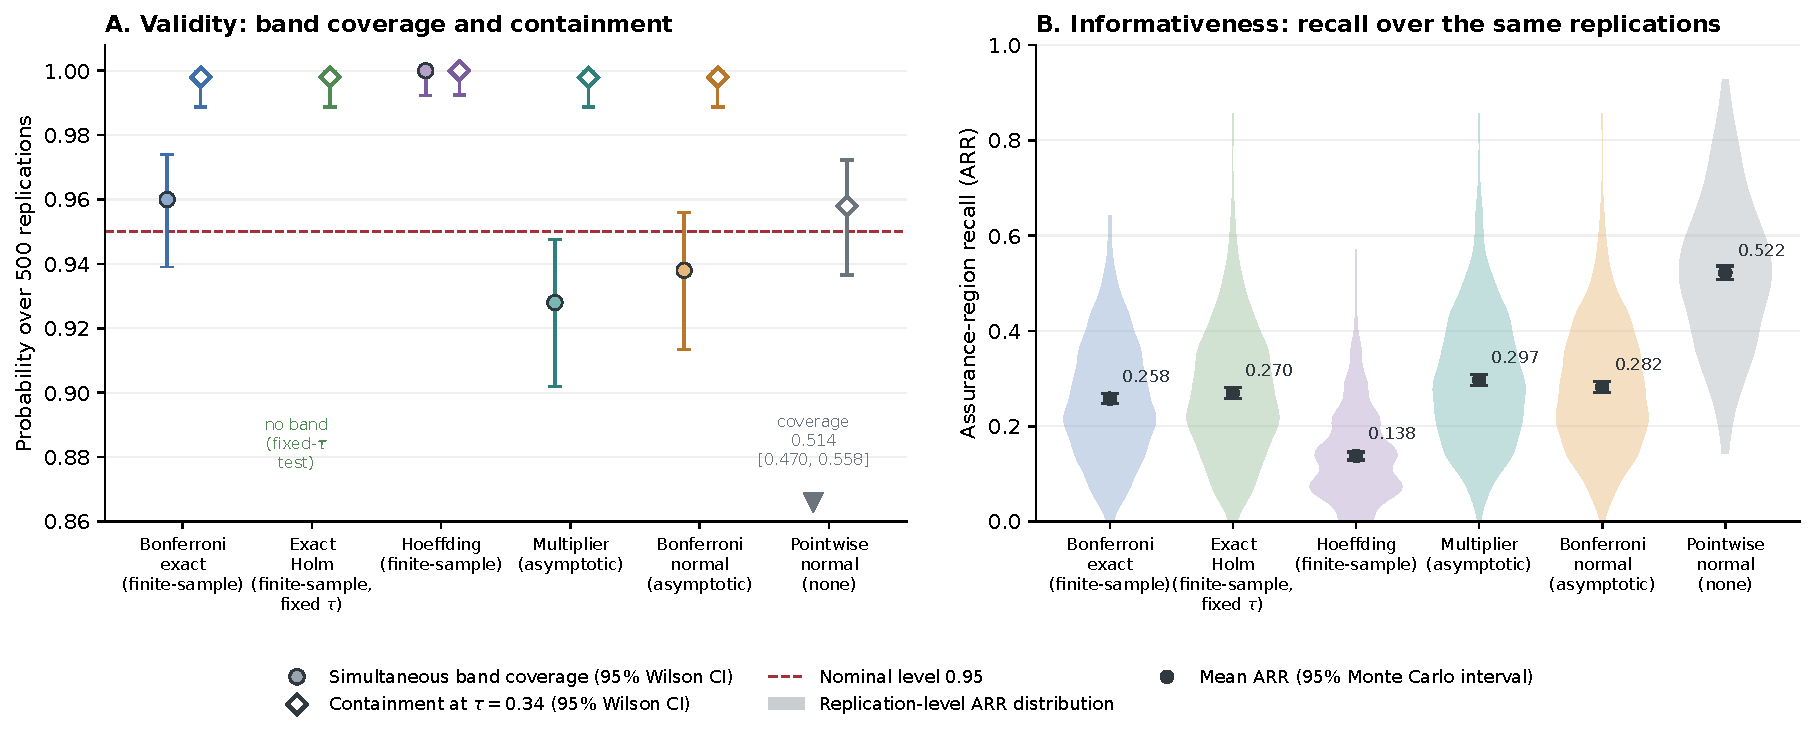
\includegraphics[width=\linewidth]{calibration_validity.pdf}
\caption{Validity and recall in the primary calibration (\CalibrationReps{} replications;
$n=1000$, $K=25$, $\tau=.34$). (A) Simultaneous band coverage (circles) and containment at
$\tau=.34$ (diamonds) with 95\% Wilson intervals; the dashed line is the nominal level. Exact
Holm has no band, and the pointwise-normal coverage lies below the plotted range, as marked.
(B) Distribution of ARR over the same replications, with means and 95\% Monte Carlo intervals.
The corresponding figure for the adverse regimes is in Appendix~\ref{app:tables}.}
\label{fig:cal}
\end{figure}

Containment stayed near one even when band coverage failed, because band failures in this
design rarely produced false certifications. Regenerating the \AnatReps{} primary replications
from the archived seeds (Appendix~\ref{app:verification}), \AnatExactSafeOnly{} of the
\AnatExactFailures{} exact-Bonferroni coverage failures missed only acceptable environments,
and only \AnatExactFalseCert{} produced a false certification at $\tau=.34$; for the multiplier,
\AnatMultSafeOnly{} of \AnatMultFailures{} failures missed only acceptable environments and
\AnatMultFalseCert{} produced a false certification (Table~\ref{tab:anatomy}). When an
unacceptable environment was missed, its upper bound usually remained between $\tau$ and its
true risk. Containment at one tolerance therefore says little about the validity of a band.

In the bounded-continuous and rare-binary designs, the Bonferroni normal and multiplier bands
have identical coverage; their coverage indicators agree in all \StressIdenticalReps{}
replications of both designs, although their certified sets differ. With independent Beta
losses, the multiplier critical value (mean \StressContMultCrit) essentially equals the
Bonferroni value \StressBonfCrit. In the rare-binary design the multiplier value is smaller
(mean \StressRareMultCrit), but failures arise in environments whose standardized errors exceed
both values; in \StressRareLowCountShare\% of the failing replications, at least one missed
environment had at most three observed errors. Both bands rely on the same studentized normal
approximation and fail when it fails.

\subsection{Power and Sample-Size Planning}
\label{sec:power}
Certification depends most directly on the distance between each risk and the tolerance. A
factorial power study therefore sets $\tau=.10$ and gives half of the $K$ environments risk
$\tau-\Delta$ and half risk $\tau+\Delta$, for $K\in\{25,100\}$,
$n\in\{250,500,1000,2000,4000,8000\}$, and $\Delta\in\{.01,.02,.03,.05\}$. Binary losses are
generated by the Gaussian copula with latent correlation $.55$, using \PowerReps{}
replications per cell and 2,000 multiplier draws. The simulated exact-Bonferroni recall agrees
with \eqref{eq:pcert} to within \PowerAnalyticMaxDev{} in every cell, which checks the
simulation and allows \eqref{eq:pcert} to be used for planning without simulation.

\begin{figure}[t]
\centering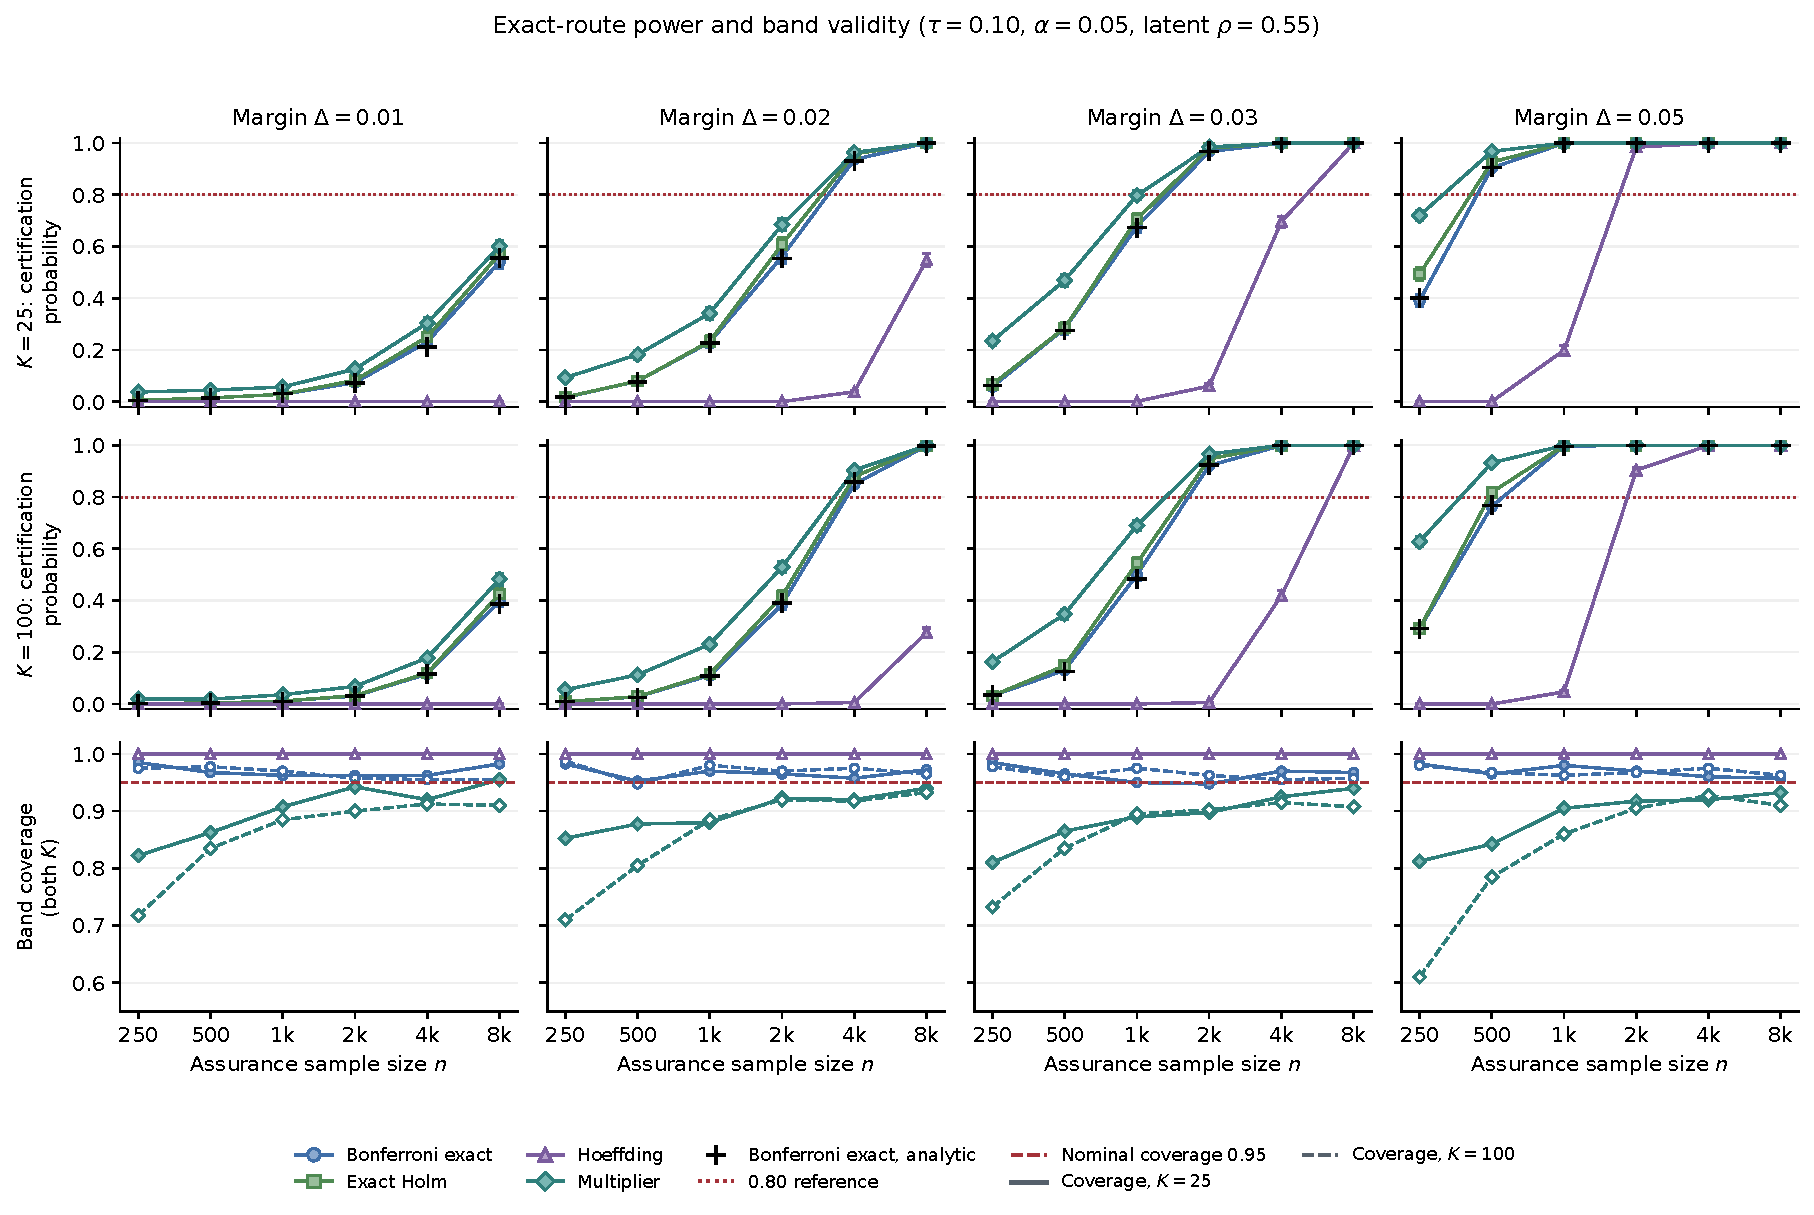
\includegraphics[width=\linewidth]{power.pdf}
\caption{Risk-margin power study ($\tau=.10$, $\alpha=.05$, latent correlation $.55$,
\PowerReps{} replications per cell). Half of the $K$ environments have risk $\tau-\Delta$ and
half $\tau+\Delta$. Top two rows: probability of certifying an environment at risk
$\tau-\Delta$ for $K=25$ and $K=100$; crosses are the closed-form exact-Bonferroni values from
\eqref{eq:pcert}, and the dotted line marks 0.8. Bottom row: simultaneous band coverage
(solid, $K=25$; dashed, $K=100$) with the nominal level 0.95. Holm has no band and is omitted
from the bottom row.}
\label{fig:power}
\end{figure}

Figure~\ref{fig:power} shows that the certification probability rises steeply once the width
of the bound falls below the margin, and reducing the margin from $.05$ to $.01$ moves this
transition by more than an order of magnitude in $n$. At $\tau=.10$, exact Bonferroni needs
\PlanExactDeltaFiveLo{} to \PlanExactDeltaFiveHi{} assurance observations, for $K$ between 25
and 500, to certify an environment with margin $.05$ with probability at least 0.8, but
\PlanExactDeltaOneLo{} to \PlanExactDeltaOneHi{} for margin $.01$. Exact Holm improved on exact
Bonferroni by at most \PowerHolmGainMax{} in certification probability, and Hoeffding needed
far larger samples than either exact procedure. The largest gain of the multiplier,
\PowerMultGainMax, occurred in the cell where its band coverage was lowest,
\PowerMultBestGainCov. Its coverage was \PowerMultCovSmallKLo--\PowerMultCovSmallKHi{} at
$n=\PowerSmallN$ with $K=\PowerKsmall$ and \PowerMultCovLargeKLo--\PowerMultCovLargeKHi{} with
$K=\PowerKlarge$, although every environment then had at least 12 expected errors, and it
remained between \PowerMultCovLargeNLo{} and \PowerMultCovLargeNHi{} at $n=\PowerLargeN$. Exact
Bonferroni coverage was at least \PowerExactCovMin, and containment was at least
\PowerMinContainment{} for every procedure (Table~\ref{tab:power-validity}).

The deficit that remains at $n=\PowerLargeN$ for $K=\PowerKlarge$ is not Monte Carlo noise. A
studentized binomial mean has a one-sided coverage error of order $n^{-1/2}$ driven by
skewness \citep{hall1992bootstrap}, and Wald limits can undercover even at large $n$
\citep{brown2001interval}. Simultaneous inference evaluates this error far in the tail, at a
per-environment level near $\alpha/K$. An exact binomial calculation for one environment with
risk $.09$ or $.11$ shows that the studentized normal upper bound at level $\alpha/K$ fails
\TailLargeKSmallNLo--\TailLargeKSmallNHi{} times as often as nominal at $n=250$ with $K=100$,
\TailLargeKLargeNLo--\TailLargeKLargeNHi{} times as often at $n=8000$ with $K=100$, and about
\TailSmallKLargeNLo{} times as often at $n=8000$ with $K=25$ (Table~\ref{tab:tail}). Larger
families therefore need larger samples before a Gaussian band attains its nominal familywise
level. The multiplier critical value is somewhat smaller than $z_{1-\alpha/K}$ because it uses
dependence, but it relies on the same approximation.

\begin{table}[t]
\centering\small\setlength{\tabcolsep}{4pt}
\caption{Assurance-sample planning at $\tau=.10$ and $\alpha=.05$ for an environment whose risk
is $\Delta$ below the tolerance. $n_{\mathrm H}=\lceil\log(K/\alpha)/(2\Delta^2)\rceil$ is the
Hoeffding width rule. The exact columns give the smallest $n$ from which the exact-Bonferroni
certification probability \eqref{eq:pcert} stays at or above the stated level; the last two
columns give the certification probability of each procedure at $n_{\mathrm H}$.}
\label{tab:power-planning}\begin{tabular}{rrrrrrr}
\toprule
 & & Hoeffding & \multicolumn{2}{c}{Exact $n$ for $P_{\mathrm{cert}}\geq$} & \multicolumn{2}{c}{$P_{\mathrm{cert}}$ at $n_{\mathrm H}$} \\
\cmidrule(lr){4-5}\cmidrule(lr){6-7}
$K$ & $\Delta$ & width $n_{\mathrm H}$ & 0.8 & 0.9 & Hoeffding & Exact \\
\midrule
25 & 0.01 & 31,074 & 12,179 & 15,138 & 0.500 & 0.999 \\
25 & 0.02 & 7,769 & 2,966 & 3,668 & 0.502 & 0.999 \\
25 & 0.03 & 3,453 & 1,285 & 1,567 & 0.498 & 1.000 \\
25 & 0.05 & 1,243 & 422 & 522 & 0.526 & 1.000 \\
100 & 0.01 & 38,005 & 14,991 & 18,277 & 0.501 & 1.000 \\
100 & 0.02 & 9,502 & 3,648 & 4,418 & 0.507 & 1.000 \\
100 & 0.03 & 4,223 & 1,573 & 1,891 & 0.501 & 1.000 \\
100 & 0.05 & 1,521 & 528 & 616 & 0.528 & 1.000 \\
500 & 0.01 & 46,052 & 18,235 & 21,837 & 0.500 & 1.000 \\
500 & 0.02 & 11,513 & 4,431 & 5,279 & 0.508 & 1.000 \\
500 & 0.03 & 5,117 & 1,905 & 2,258 & 0.510 & 1.000 \\
500 & 0.05 & 1,843 & 626 & 741 & 0.521 & 1.000 \\
\bottomrule
\end{tabular}

\end{table}

Table~\ref{tab:power-planning} turns \eqref{eq:pcert} into a planning rule. The exact
requirement for probability 0.8 is \PlanRatioMin--\PlanRatioMax{} of the Hoeffding width rule
$n_{\mathrm H}$, and at $n_{\mathrm H}$ the Hoeffding procedure itself certifies such an
environment with probability only \PlanHoeffProbMin--\PlanHoeffProbMax: when the width equals
the margin, an estimate equal to the true risk lies exactly on the certification boundary.
Planning by certification probability rather than by width both reduces the required sample
and targets the quantity of practical interest.

Dependence between environments matters less than the margin. In a sensitivity study with 300
replications per setting, varying $n\in\{500,1000,5000\}$ at latent correlation $.55$ and
$\rho\in\{.10,.55,.90\}$ at $n=1000$ (Figure~\ref{fig:sensitivity} and
Table~\ref{tab:gains} in Appendix~\ref{app:tables}), the paired ARR gain of the multiplier over
Bonferroni normal was negligible at low correlation and larger at high correlation. Against
exact Bonferroni the gain ranged from \GainExactMin{} to \GainExactMax{} and was largest at
$\rho=.90$, where the multiplier coverage, \SensMultCovHighRho, was also adequate; at $n=500$
its coverage was \SensMultCovSmallN. Strong dependence is therefore the regime in which the
efficiency of the multiplier is both largest and best supported.

\subsection{Fitted Pipelines and Missingness Mechanisms}
\label{sec:nested}
\label{sec:missing}
The fitted-pipeline experiment uses \NestedReps{} independent refits. Each generates 1,200
training rows, 400 source-calibration rows for ATC, 1,000 assurance rows, and
\num{\ReferenceN} separate reference rows. Ten Gaussian covariates have AR(1) covariance
$\Sigma$ with parameter $.35$, and outcomes follow
\begin{equation}
\Pp(Y=1\mid X)=\operatorname{expit}\left[1.5\{.75X_0-.65X_1+.45X_2
+ .55X_0X_1-.35X_2^2+.20X_3\}\right].
\label{eq:dgp}
\end{equation}
A fixed normalized direction $\mathbf v\propto(.8,-.6,.4,.2,0,\ldots,0)$ induces the mean
shift $s\,\mathbf C\mathbf v$, where $\Sigma=\mathbf C\mathbf C^\top$ is the Cholesky
factorization. The grid has $m\in\{0,.1,.2,.3\}$ and $s\in\{0,.15,.30,.45\}$, with $\tau=.35$.
Feature $X_0$ remains observed, and the severity $m$ is the missingness rate among the other
nine features; imputation uses training means. The two pipelines are standardized logistic
regression (LR) and histogram gradient boosting (HGB; 60 iterations, 15 maximum leaves,
learning rate $.08$). The same base rows, label uniforms, and missingness randomness are used
across models and environments. Each model is certified separately over its own
16-environment family, so no joint statement over the two models, and hence no
model-selection guarantee, is claimed.

The independent reference mean $\widetilde R_k$ is itself uncertain. Simultaneous two-sided
exact binomial intervals $[a_k,b_k]$ allocate total error $.01$ over the reference risks of
both models within each refit. Cells with $b_k\leq\tau$ are confirmed acceptable, cells with
$a_k>\tau$ are confirmed unacceptable, and all others are ambiguous. Then
\begin{equation}
\begin{aligned}
C^- &=\mathbb I\{\text{all certified cells are confirmed acceptable}\},\\
C^+ &=\mathbb I\{\text{no certified cell is confirmed unacceptable}\}
\end{aligned}
\label{eq:reference}
\end{equation}
satisfy $C^-\leq C\leq C^+$ on the reference-coverage event. We report the means of these
endpoints as a reference bracket, not as confidence limits for a coverage probability; the
reference budget is per refit, not a joint guarantee over refits.

The missingness study uses \MissingnessReps{} logistic-regression refits with the same design
and compares missing completely at random (MCAR), MAR, missing not at random (MNAR), and
structured missingness. MAR depends only on the always-observed $X_0$, whereas MNAR depends on
the latent value of the feature being hidden. Logistic intercepts solve a population Gaussian
expectation equation for the target marginal missingness, using 64-node Gaussian quadrature,
and are fixed before evaluation rather than normalized with assurance rows. Under each mean
shift, the MAR and MNAR models are applied to the covariate centered at the known shifted
mean of that environment, so the marginal missingness stays at $m$ in every environment;
averaged over environments and refits, the realized fractions differ from their nominal values
by at most $.0003$. Structured missingness makes features 1--3 missing together, each with
marginal severity $m$. Reference intervals allocate error $.01$ over the four mechanisms
within each refit.

\begin{table}[t]
\centering\small\setlength{\tabcolsep}{4pt}
\caption{Fitted pipelines and missingness mechanisms. Reference containment uses the
reference means, with 95\% Wilson intervals; the reference bracket averages $[C^-,C^+]$ in
\eqref{eq:reference} and reflects ambiguity in the reference risks, not Monte Carlo uncertainty.
ARR uses reference means. Panel A: \NestedReps{} nested refits; LR denotes logistic regression
and HGB histogram gradient boosting, each certified over its own 16-environment family. Panel B:
multiplier results for \MissingnessReps{} logistic-regression refits under each mechanism;
ambiguous cells are averaged over the 16 environments per refit.}
\label{tab:nested}\label{tab:missing}
\begin{tabular}{l}Panel A. Nested refits\end{tabular}\\[2pt]
\begin{tabular}{llrrr}
\toprule
Model & Method & Reference containment [95\% CI] & ARR & Reference bracket \\
\midrule
LR & Bonferroni exact & 1.000 [0.981, 1.000] & 0.139 & [0.970, 1.000] \\
LR & Exact Holm & 1.000 [0.981, 1.000] & 0.167 & [0.955, 1.000] \\
LR & Hoeffding & 1.000 [0.981, 1.000] & 0.047 & [0.995, 1.000] \\
LR & Multiplier & 1.000 [0.981, 1.000] & 0.237 & [0.940, 1.000] \\
LR & Bonferroni normal & 1.000 [0.981, 1.000] & 0.167 & [0.960, 1.000] \\
HGB & Bonferroni exact & 1.000 [0.981, 1.000] & 0.631 & [1.000, 1.000] \\
HGB & Exact Holm & 1.000 [0.981, 1.000] & 0.732 & [1.000, 1.000] \\
HGB & Hoeffding & 1.000 [0.981, 1.000] & 0.395 & [1.000, 1.000] \\
HGB & Multiplier & 1.000 [0.981, 1.000] & 0.735 & [1.000, 1.000] \\
HGB & Bonferroni normal & 1.000 [0.981, 1.000] & 0.669 & [1.000, 1.000] \\
\bottomrule
\end{tabular}
\\[8pt]
\begin{tabular}{l}Panel B. Missingness mechanisms (multiplier)\end{tabular}\\[2pt]
\begin{tabular}{lrrrr}
\toprule
Mechanism & Reference containment & Reference bracket & ARR & Ambiguous cells \\
\midrule
MCAR & 1.000 [0.963, 1.000] & [0.940, 1.000] & 0.211 & 1.83 \\
MAR & 1.000 [0.963, 1.000] & [0.990, 1.000] & 0.249 & 0.28 \\
MNAR & 1.000 [0.963, 1.000] & [1.000, 1.000] & 0.303 & 0.00 \\
Structured & 1.000 [0.963, 1.000] & [0.930, 1.000] & 0.232 & 0.98 \\
\bottomrule
\end{tabular}

\end{table}

\begin{figure}[t]
\centering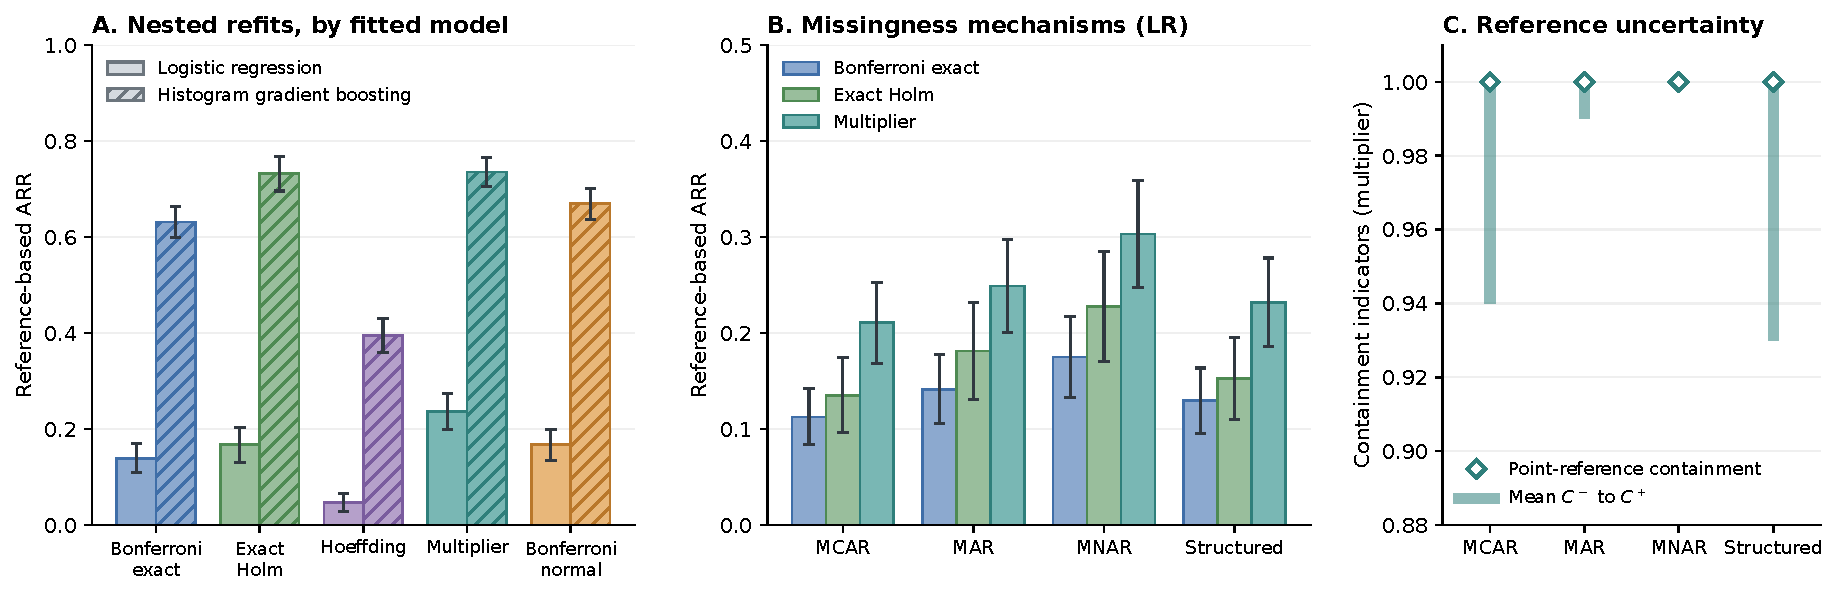
\includegraphics[width=\linewidth]{pipelines_missingness.pdf}
\caption{Fitted pipelines and missingness mechanisms. (A) Reference-based ARR across
\NestedReps{} nested refits for logistic regression (plain) and histogram gradient boosting
(hatched). (B) Reference-based ARR for three procedures under four missingness mechanisms
(\MissingnessReps{} logistic-regression refits). Error bars in (A) and (B) are approximate 95\%
intervals based on the replication-level MCSE. (C) Point-reference containment of the
multiplier (diamonds) and the mean reference bracket $[C^-,C^+]$ (bars), which is not a
confidence interval.}
\label{fig:nested}\label{fig:missing}
\end{figure}

Table~\ref{tab:nested} and Figure~\ref{fig:nested} show that the fitted pipeline mattered more
than the valid procedure that certified it. Exact Bonferroni recovered 0.139 of the
reference-acceptable cells for logistic regression and 0.631 for histogram gradient boosting,
whereas the two exact procedures differed by about 0.10 or less within either model, and
exact Holm and the multiplier had nearly equal recall for HGB. Point-reference containment was
1.000 for every procedure, model, and mechanism, but this is not proof of perfect
containment. For logistic regression, certified cells near the tolerance were sometimes
ambiguous under the reference intervals, so the lower endpoint of the bracket ranged from
0.940 to 0.995 across procedures. HGB had no ambiguous cells in these runs, so its favorable
recall is a result for this fitted-model regime rather than evidence about difficult
near-boundary cases. In the missingness study the lower endpoint ranged from 0.930 to 1.000 and
equaled one only for MNAR, the mechanism with no ambiguous cells; these results concern the
chosen parameterizations and do not imply that MNAR is generally easier than MCAR.

For comparison, ATC with the maximum class probability as its confidence score, a
source-calibrated strict threshold, and tied scores handled jointly predicted the reference
risks with mean absolute error 0.031 for logistic regression and 0.030 for histogram gradient
boosting (bias $-0.012$ and $-0.014$; root mean squared error 0.033 and 0.032). ATC uses no
target labels, whereas the certification procedures use labeled assurance losses, so this is
a descriptive comparison of a neighboring task rather than a comparison of equal guarantees.

\section{Real Data Analyses}
\label{sec:realdata}

\subsection{Wisconsin Diagnostic Breast Cancer Data}
\label{sec:wdbc}
The WDBC data contain 569 observations. A fixed stratified 65/35 split gives 369 training
rows and 200 assurance rows. The fixed models are standardized logistic regression, an Extra
Trees ensemble with 500 trees, and histogram gradient boosting. Training means impute missing
values, and Gaussian feature noise is scaled by training standard deviations. One noise matrix
and one uniform missingness matrix are shared across stress conditions and models. The primary
family crosses $m\in\{0,.05,.10,.20,.30,.40\}$ with $s\in\{0,.10,.20,.30,.40,.50\}$, the
multiplier uses 5,000 draws, and the tolerances $\tau=.08$ and $.10$ are illustrative, not
medical standards.

\begin{table}[t]
\centering\small
\caption{WDBC results for separate model-specific 36-environment families. The nominal
observed risk is descriptive.}
\label{tab:wdbc}\begin{tabular}{llrrr}
\toprule
Model & Method & Nominal risk & Certified $\tau=.08$ & Certified $\tau=.10$ \\
\midrule
LR & Bonferroni exact & 0.010 & 15/36 & 23/36 \\
LR & Exact Holm & 0.010 & 15/36 & 27/36 \\
LR & Multiplier & 0.010 & 23/36 & 30/36 \\
LR & Bonferroni normal & 0.010 & 20/36 & 29/36 \\
Extra Trees & Bonferroni exact & 0.035 & 0/36 & 9/36 \\
Extra Trees & Exact Holm & 0.035 & 0/36 & 9/36 \\
Extra Trees & Multiplier & 0.035 & 9/36 & 19/36 \\
Extra Trees & Bonferroni normal & 0.035 & 2/36 & 17/36 \\
HGB & Bonferroni exact & 0.045 & 0/36 & 2/36 \\
HGB & Exact Holm & 0.045 & 0/36 & 2/36 \\
HGB & Multiplier & 0.045 & 2/36 & 14/36 \\
HGB & Bonferroni normal & 0.045 & 0/36 & 12/36 \\
\bottomrule
\end{tabular}

\end{table}
\begin{figure}[t]
\centering\includegraphics[width=\linewidth]{wdbc.pdf}
\centering\includegraphics[width=\linewidth]{wdbc_upc.pdf}
\caption{WDBC assurance results for the three models. Top: certification maps over the
missingness--shift grid; green cells are certified at $\tau=.08$, yellow cells only at
$\tau=.10$, and red cells at neither. Bottom: observed risk (solid) and exact Bonferroni
one-sided familywise upper bounds (dashed) against added MCAR missingness, with one curve per
shift level; the dotted line marks the tolerance.}
\label{fig:wdbc}
\end{figure}

Logistic regression has the lowest observed error in this split, and exact Bonferroni
certified 15 of its 36 conditions at $\tau=.08$ and 23 at $\tau=.10$ (Table~\ref{tab:wdbc} and
Figure~\ref{fig:wdbc}). The counts depend strongly on the procedure and the tolerance. They are
separate model-specific simultaneous statements, so choosing a model by comparing them does
not confer joint model-selection coverage. The perturbations are synthetic and do not
represent observed temporal or inter-hospital shifts, and a single split cannot estimate the
true region, ARR, or a coverage probability. Equally spaced $4\times4$, $6\times6$, and
$10\times10$ grids for logistic regression are reported in Table~\ref{tab:grid}; certified grid
fractions cannot be read as continuous areas without a design measure or a smoothness
argument, and no grid was selected retrospectively.

\subsection{MIMIC-IV Mortality Prediction}
\label{sec:mimic}
We applied the procedure to credentialed MIMIC-IV v3.1 data \citep{mimic31,johnson2023mimic}
to examine whether it can be carried through on a large electronic health record cohort with
approximate temporal grouping and native missingness. We do not establish or quantify
covariate or outcome shift across these groups, and neither risk target constitutes a
clinically validated deployment rule.

\subsubsection{Cohort and Design}
The raw join contained 546,028 admissions. After retaining valid adult admissions and the first
eligible admission per patient, 223,452 patients remained. Admission-aligned temporal
intervals placed 106,864 patients in the source cohort and 35,114 in deployment; 81,474
admissions whose assignment was ambiguous under the padded interval rule were excluded. This
exclusion is a deterministic function of each patient's own interval metadata and fixed
cutoffs and does not couple patients, so the retained observations preserve the
independent-row construction of Lemma~\ref{lem:rows}. The source cohort was split into 85,491
fitting observations and a 21,373-observation source holdout. The outcome was in-hospital
mortality. Predictors were age, an age-topcoding indicator, gender, admission type, admission
location, insurance, marital status, and race; no laboratory measurements, vital signs,
medications, or ICU time series were used, and identifiers, outcome flags, death or discharge
times, and length of stay were excluded.

MIMIC-IV shifts dates separately for each patient. We therefore align each admission to the
patient anchor year, form approximate admission intervals, pad interval endpoints by one year,
and restrict them to the declared v3.1 coverage. The resulting labels are approximate ordering
intervals rather than shared calendar periods and should not be read as secular trends. The
source period ends by 2016, and the deployment domains are the approximate intervals
2017--2021, 2018--2022, 2019--2022, 2020--2022, 2021--2022, and 2022--2022. The labels may
overlap in calendar time, but each patient contributes to one domain. The grouped construction
of Section~\ref{sec:natural-groups} accommodates unequal domain sizes, and common-row inference
preserves dependence across the model and missingness conditions evaluated on the same
patients. Treating patients as independent within a domain ignores shared period effects, such
as waves of admissions or changes in practice; the bounds are conditional on that assumption.

Unweighted logistic regression and histogram gradient boosting were fitted on the source
training cohort, and an always-survive classifier was retained for comparison. Added MCAR
feature missingness took the levels $m\in\{0,.10,.20,.30\}$, with native missingness recorded
separately. The three models, six domains, and four missingness levels define one
72-condition family. Before certification we fixed $\alpha=.05$, 5,000 multiplier draws, and
a minimum domain size of 200, and all four inferential procedures were applied to the same
family.

\subsubsection{Misclassification Risk}
The tolerance $\tau=.35$ for 0--1 risk was fixed before deployment outcomes were examined. It
was chosen as a deliberately loose threshold for executing the procedure, not as a clinically
acceptable error rate, and because the source-holdout risks were available when it was
finalized, this specification is not a prospective clinical requirement. The source-holdout
risks were 0.0184 for logistic regression, 0.0185 for histogram gradient boosting, and 0.0184
for the always-survive classifier. Five domains met the minimum size, giving 60 eligible
conditions; the 2022--2022 domain contained only 32 patients, so its 12 conditions were
retained as ineligible. All 60 eligible conditions were certified by all four procedures. The
largest exact-Bonferroni upper risk was 0.0474, the largest Hoeffding bound was 0.1044, and the
multiplier critical value was 2.538 with largest upper bound 0.0465
(Table~\ref{tab:mimic} and Figure~\ref{fig:mimic}, top).

\begin{table}[t]
\centering\small
\caption{MIMIC-IV temporal domains under the misclassification-risk specification. Mortality
prevalence, logistic-regression risk, AUROC, and AUPRC are at zero added missingness. ``Max
$U$'' is the largest exact-Bonferroni upper risk across the three models and four missingness
levels in that domain, and the last column gives certified/total conditions.
$^\dagger$The 2022--2022 domain is ineligible because $n<200$; its conditions remain in the
family but are not certified, and AUROC and AUPRC are not reported for this one-death domain.}
\label{tab:mimic}
\begin{tabular}{lrrrrrrc}
\toprule
Interval & $n$ & Mort. & LR risk & AUROC & AUPRC & Max $U$ & Cert. \\
\midrule
2017--2021 & 2,312 & 0.006 & 0.006 & 0.805 & 0.099 & 0.014 & 12/12 \\
2018--2022 & 1,645 & 0.007 & 0.007 & 0.871 & 0.069 & 0.020 & 12/12 \\
2019--2022 & 29,419 & 0.037 & 0.039 & 0.844 & 0.176 & 0.047 & 12/12 \\
2020--2022 & 1,282 & 0.010 & 0.010 & 0.914 & 0.104 & 0.024 & 12/12 \\
2021--2022 & 424 & 0.012 & 0.012 & 0.951 & 0.173 & 0.039 & 12/12 \\
2022--2022 & 32 & 0.031 & 0.031 & -- & -- & -- & 0/12$^\dagger$ \\
\bottomrule
\end{tabular}

\end{table}

\begin{figure}[t]
\centering
\includegraphics[width=\linewidth]{mimic_sar_decision_map.pdf}\\[4pt]
\includegraphics[width=\linewidth]{mimic_class_sensitive_sar.pdf}
\caption{MIMIC-IV assurance maps using exact Clopper--Pearson Bonferroni upper risks. Columns
add 0--30\% MCAR feature missingness and rows are approximate admission intervals. Top:
misclassification risk at $\tau=.35$; the 2022--2022 interval ($n=32<200$) is withheld from
certification. Bottom: false-negative risk at $\tau_{\mathrm{FN}}=.20$, equivalent to a
required sensitivity of at least 0.80, with thresholds calibrated on the source holdout and then
fixed; yellow cells have observed risk at or below the tolerance but an upper bound above it,
red cells have observed risk above the tolerance, and gray cells have too few positive cases.
Green cells are certified. The maps report statistical support for the prespecified criteria,
not clinical safety.}
\label{fig:mimic}\label{fig:mimic-fn}
\end{figure}

This specification exposes a limitation of thresholded 0--1 loss for a rare outcome. At zero
added missingness, logistic-regression AUROC ranged from 0.805 to 0.951 across the eligible
domains, yet sensitivity at the default 0.5 threshold was zero in four domains and 0.049 in
2019--2022. The always-survive classifier was also certified in every eligible condition
because mortality was rare, and this does not depend on the loose value $\tau=.35$: it is
certified in every eligible condition at any tolerance above \MimicAlwaysFull{}
(Section~\ref{sec:profiles}). The certification is internally valid for the specified loss and
tolerance but says little about the detection of deaths.

\subsubsection{False-Negative Risk}
To make the target informative for the minority outcome, a secondary specification bounds the
false-negative risk $R_{\mathrm{FN}}(e)=\Pr\{\widehat Y=0\mid Y=1,e\}$, analyzed as in
Section~\ref{sec:classcond}. It was introduced after the primary analysis had shown zero
sensitivity, so it is prespecified only relative to its own deployment results. Before those
results were computed, we fixed $\tau_{\mathrm{FN}}=.20$, corresponding to a sensitivity of at
least 0.80; this requirement is interpretable but is not claimed to be a clinical standard. For
each learned model, the largest threshold attaining sensitivity 0.80 was selected on the
independent source holdout and then fixed: 0.0217 for logistic regression and 0.0227 for
histogram gradient boosting, with source sensitivity 0.802 and specificity 0.747 and 0.749,
respectively. Because the source holdout is disjoint from the deployment cohort, this
calibration does not reuse deployment outcomes. Exact Clopper--Pearson Bonferroni was the
primary procedure and exact Holm a secondary check. A minimum of two positive cases per domain
was fixed before certification, so the one-death 2022--2022 domain is ineligible.

Positive-case counts in the six domains were 14, 12, 1,092, 13, 5, and 1. Of the 60 eligible
conditions, exact Bonferroni certified 3, all for histogram gradient boosting in 2019--2022 at
0\%, 10\%, and 20\% added missingness, with observed sensitivities 0.852, 0.848, and 0.845 and
upper false-negative bounds 0.1855, 0.1895, and 0.1925. At 30\% missingness the same model had
observed sensitivity 0.818 but upper bound 0.218 and was not certified. Logistic regression
and the always-survive classifier each certified 0 of 20 conditions, and exact Holm certified
the same three conditions and no others (Figure~\ref{fig:mimic}, bottom).

The 3-of-60 count describes where the data contain enough positive cases to support a
familywise statement rather than ranking the models across domains. For false-negative risk
the effective sample size of a domain is its number of deaths $n_+$. With Bonferroni
correction over the full \EssK-condition family, zero false negatives among $n_+$ deaths give
the smallest attainable upper bound, $1-(\alpha/K)^{1/n_+}$, so certification at
$\tau_{\mathrm{FN}}=.20$ is impossible unless $n_+\geq\EssZeroDeaths$. Even zero false
negatives among 14 deaths give an upper bound of \EssZeroFNUpperFourteen, a lower sensitivity
bound of only \EssBestLowerFourteen. Four of the five eligible domains contain
\EssSmallDeathsMin--\EssSmallDeathsMax{} deaths, so none of their conditions could be certified
even with perfect observed sensitivity (Table~\ref{tab:mimic-ess}), and the secondary
analysis is in effect a single-domain result. In the 2019--2022 domain, with \EssLargeDeaths{}
deaths, the exact lower bounds separate the two models: histogram gradient boosting has lower
sensitivity bound 0.815 at zero added missingness and is certified, whereas logistic regression
has 0.766 and is not. Applying \eqref{eq:pcert} to the false-negative rate, a domain whose true
sensitivity is 0.90 needs about \EssDeathsNinety{} deaths for an 80\% probability of
certification, \EssDeathsNinetyFive{} at true sensitivity 0.95, and \EssDeathsEightyFive{} at
0.85 (\EssDeathsEightyFiveNinety{} for a 90\% probability). At the mortality prevalence of the
four small domains, \EssPrevLo--\EssPrevHi\%, \EssDeathsNinety{} deaths correspond to roughly
\EssAdmissionsLo{} to \EssAdmissionsHi{} admissions per domain, so the number of positive cases
should be planned before the analysis.

\IfFileExists{generated/mimic_operating.tex}{%
\begin{table}[t]
\centering\small\setlength{\tabcolsep}{4pt}
\caption{MIMIC-IV false-negative-risk specification by domain. Panel A: effective sample size.
``Best lower sens.'' is the exact lower sensitivity bound that zero false negatives would give,
$1-(\alpha/K)^{1/n_+}$ with $K=\EssK$, and certification at $\tau_{\mathrm{FN}}=.20$ requires it
to be at least 0.80; observed sensitivities and their exact familywise lower bounds (brackets)
are at 0\% added missingness, and certified counts are over the four missingness levels.
Panel B: descriptive operating characteristics of the fixed thresholds at zero added
missingness, which carry no inferential guarantee.}
\label{tab:mimic-ess}\label{tab:mimic-operating}
\begin{tabular}{l}Panel A. Effective sample size and certification\end{tabular}\\[2pt]
\begin{tabular}{lrrcrrrr}
\toprule
 & & Best lower & Can & \multicolumn{2}{c}{Sensitivity [lower bound]} & \multicolumn{2}{c}{Certified} \\
\cmidrule(lr){5-6}\cmidrule(lr){7-8}
Interval & Deaths & sens. & certify? & LR & HGB & LR & HGB \\
\midrule
2017--2021 & 14 & 0.595 & no & 0.286 [0.031] & 0.357 [0.056] & 0/4 & 0/4 \\
2018--2022 & 12 & 0.546 & no & 0.500 [0.105] & 0.667 [0.205] & 0/4 & 0/4 \\
2019--2022 & 1,092 & 0.993 & yes & 0.807 [0.766] & 0.852 [0.815] & 0/4 & 3/4 \\
2020--2022 & 13 & 0.572 & no & 0.615 [0.184] & 0.769 [0.302] & 0/4 & 0/4 \\
2021--2022 & 5 & 0.234 & no & 0.800 [0.111] & 1.000 [0.234] & 0/4 & 0/4 \\
2022--2022 & 1 & -- & no & -- & -- & -- & -- \\
\bottomrule
\end{tabular}
\\[8pt]
\begin{tabular}{l}Panel B. Operating characteristics\end{tabular}\\[2pt]
\input{generated/mimic_operating.tex}
\end{table}

Sensitivity alone does not describe the cost of a threshold (Table~\ref{tab:mimic-operating},
Panel B). In the 2019--2022 domain at zero added missingness, histogram gradient boosting had
sensitivity 0.852, compared with 0.807 for logistic regression, but generated 397.6 rather than
295.7 alerts per 1,000 admissions, with positive predictive values of 0.080 and 0.101. Meeting
the sensitivity requirement therefore does not by itself establish an acceptable alert burden
or clinical utility.
}{%
\begin{table}[t]
\centering\small\setlength{\tabcolsep}{4pt}
\caption{Effective sample size of the MIMIC-IV false-negative-risk specification. ``Best lower
sens.'' is the exact lower sensitivity bound that zero false negatives would give,
$1-(\alpha/K)^{1/n_+}$ with $K=\EssK$, and certification at $\tau_{\mathrm{FN}}=.20$ requires it
to be at least 0.80; observed sensitivities and their exact familywise lower bounds (brackets)
are at 0\% added missingness, and certified counts are over the four missingness levels.}
\label{tab:mimic-ess}
\begin{tabular}{lrrcrrrr}
\toprule
 & & Best lower & Can & \multicolumn{2}{c}{Sensitivity [lower bound]} & \multicolumn{2}{c}{Certified} \\
\cmidrule(lr){5-6}\cmidrule(lr){7-8}
Interval & Deaths & sens. & certify? & LR & HGB & LR & HGB \\
\midrule
2017--2021 & 14 & 0.595 & no & 0.286 [0.031] & 0.357 [0.056] & 0/4 & 0/4 \\
2018--2022 & 12 & 0.546 & no & 0.500 [0.105] & 0.667 [0.205] & 0/4 & 0/4 \\
2019--2022 & 1,092 & 0.993 & yes & 0.807 [0.766] & 0.852 [0.815] & 0/4 & 3/4 \\
2020--2022 & 13 & 0.572 & no & 0.615 [0.184] & 0.769 [0.302] & 0/4 & 0/4 \\
2021--2022 & 5 & 0.234 & no & 0.800 [0.111] & 1.000 [0.234] & 0/4 & 0/4 \\
2022--2022 & 1 & -- & no & -- & -- & -- & -- \\
\bottomrule
\end{tabular}

\end{table}

\noindent\fbox{\parbox{\dimexpr\linewidth-2\fboxsep-2\fboxrule\relax}{\small Author note (remove
before submission): generated/mimic\_operating.tex was not found, so Panel B (deployment
specificity, positive predictive value, and alerts per 1,000 admissions) is omitted. Upload the
locally generated file to restore it.}}
}

The two specifications are reported as separate assurance statements. No adjustment for
multiplicity across specifications is claimed, neither is selected post hoc as the better result, and they
should not be combined into one familywise statement. The contrast between them is the
substantive lesson: inference cannot repair an inadequate loss, threshold, or tolerance, but
changing the scientific target changes the assurance question transparently.

\subsection{Tolerance--Certification Profiles}
\label{sec:profiles}
A certified count describes a single tolerance. Because a simultaneous band covers every
tolerance at once (Proposition~\ref{prop:finite}), the profile $\tau\mapsto|\widehat\A_\tau|/K$
computed from one exact-Bonferroni band is covered by the same $1-\alpha$ statement. The
display resembles the risk--coverage curves used to evaluate reject-option classifiers
\citep{franc2023reject}, but it is indexed by environments rather than instances, and it
describes sensitivity to the tolerance rather than a device for choosing it. Exact Holm is
omitted because its guarantee holds only at a fixed tolerance.

\begin{figure}[t]
\centering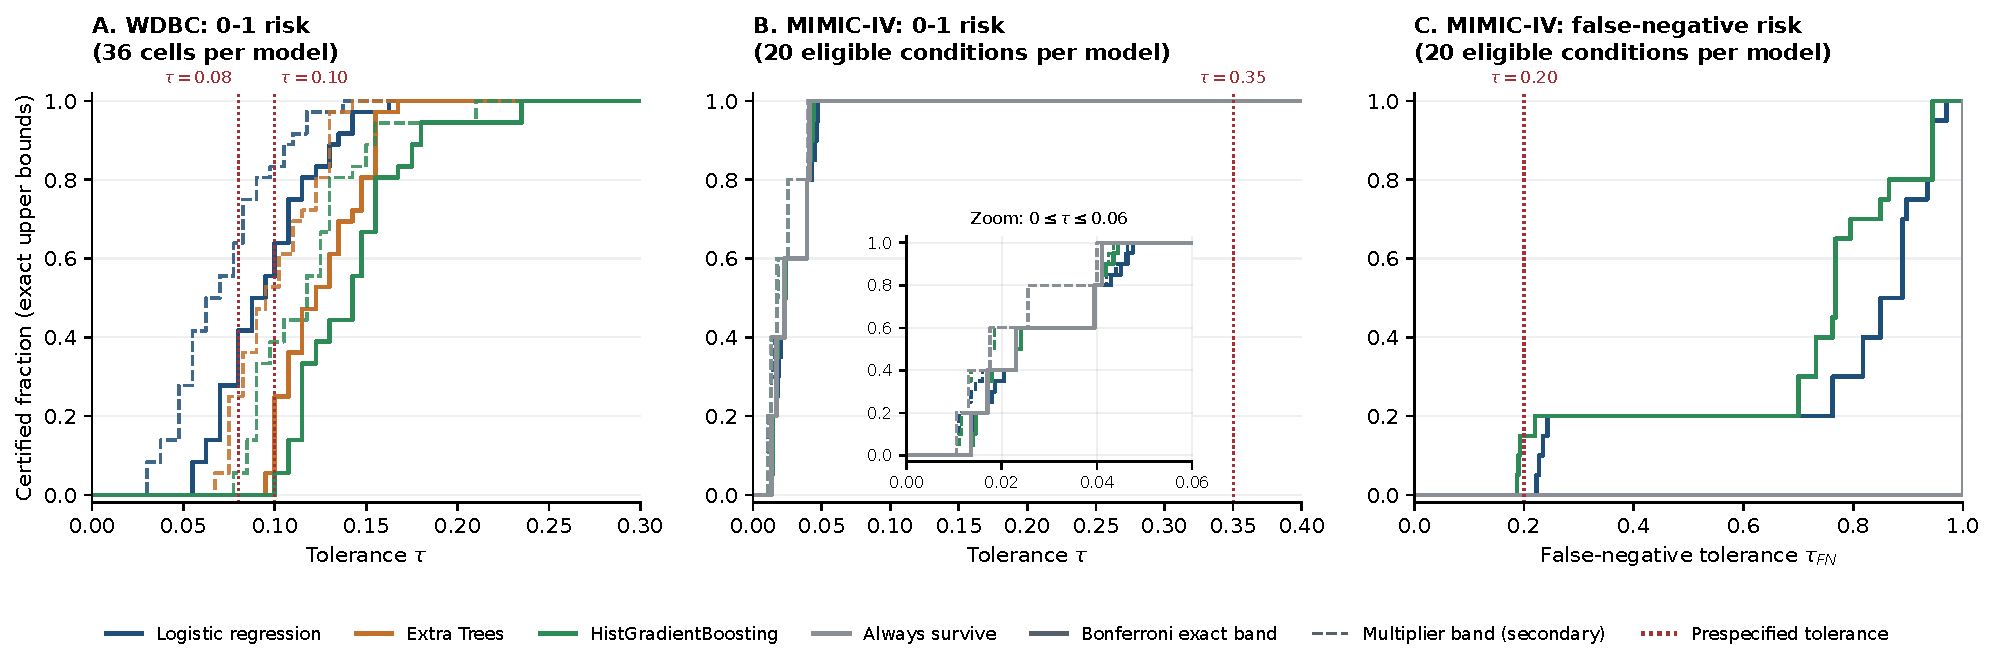
\includegraphics[width=\linewidth]{tolerance_profiles.pdf}
\caption{Tolerance--certification profiles: the fraction of each model's family certified at
tolerance $\tau$ by one simultaneous band, using exact Clopper--Pearson Bonferroni bounds
(solid) and, where available, the multiplier band (dashed). Dotted vertical lines mark the
prespecified tolerances. (A) WDBC, 36 cells per model. (B) MIMIC-IV misclassification risk, 20
eligible conditions per model; the inset enlarges $0\leq\tau\leq0.06$. (C) MIMIC-IV
false-negative risk.}
\label{fig:profiles}
\end{figure}

For WDBC (Figure~\ref{fig:profiles}A), logistic regression certifies its first cell at
$\tau=\WdbcExactFirstLR$ and all 36 at \WdbcExactFullLR, whereas histogram gradient boosting
needs \WdbcExactFullHGB{} for all 36. The ordering of the three models is the same at every
tolerance up to $.15$, but both prespecified tolerances fall at the onset or on the steep part
of the curves, which is why the WDBC counts change so much between $\tau=.08$ and $.10$. For
MIMIC-IV misclassification risk, every curve, including the always-survive classifier, reaches
one below $\tau=.05$. For false-negative risk the 2019--2022 conditions become certified as the
tolerance increases from \ProfileFnLargeMin{} to \ProfileFnLargeMax, while no condition in the
four small domains is certified below \ProfileFnSmallMinUpper, a value no practical sensitivity
requirement would allow. The conclusion that only the 2019--2022 domain supports a
class-sensitive certification therefore holds for every plausible tolerance.

\section{Discussion}
\label{sec:discussion}
For binary losses, we recommend exact Clopper--Pearson Bonferroni or exact Holm as the default
when the sampling assumptions are defensible. Sparse counts strengthen this recommendation, but
a minimum expected error count is not sufficient: the multiplier band undercovered at
$n=\PowerSmallN$ with at least 12 expected errors in every environment, more severely for
$K=\PowerKlarge$ than for $K=\PowerKsmall$, and it still undercovered at $n=\PowerLargeN$ with
$K=\PowerKlarge$. The multiplier remains useful as a dependence-aware secondary analysis,
particularly under strong dependence, where its gain was largest and its coverage adequate.
For nonbinary bounded losses, a bounded-loss inequality is appropriate when conservatism is
acceptable. Any use of the multiplier should be accompanied by finite-sample validation in a
comparable design. Exact procedures have the further advantage that their decisions are
deterministic functions of the error counts, whereas multiplier decisions near the boundary
can change with the bootstrap draws (Appendix~\ref{app:verification}).

Because certification depends mainly on the margin between each risk and the tolerance, the
assurance sample should be planned for a target certification probability at a stated margin,
using \eqref{eq:pcert}, rather than for a band width. For class-conditional risks the relevant
sample size is the number of cases in the conditioning class; for the MIMIC-IV false-negative
target, that means deaths per domain rather than admissions. Grid size is a further
constraint. The direct multiplier implementation costs $O(BnK)$ operations, and the
conditional-covariance alternative costs $O(nK^2+K^3+BK^2)$ with $O(K^2)$ storage
(Appendix~\ref{app:runtime}), which reinforces the recommendation to keep stress axes focused
or to screen a larger family with an independent pilot.

Selection and reuse also need care. A fixed band supports all tolerances simultaneously,
including one inspected afterward, but this does not justify defining an operational
requirement retroactively. Changing models, losses, or families, or choosing the most
favorable unadjusted procedure after seeing the assurance losses, requires protection over the
enlarged selection problem. Repeated 95\% checks are not a time-uniform 95\% statement; a
simple conservative extension uses fresh assurance data at round $t$ and level
$\alpha_t=\alpha/[t(t+1)]$, so that $\sum_{t\geq1}\alpha_t=\alpha$ and a union bound controls any
erroneous certification over all rounds, although this does not give efficient sequential
region learning.

The study has several limitations. The inferential components are standard, and no
optimality result, minimax recovery rate, or efficient adaptive grid is established. The
continuous extension depends on external smoothness, and unknown shifts, causal
transportability, unbounded heavy-tailed losses, and adversarial adaptation are outside its
scope. Reference-risk uncertainty persists near the tolerance even with \num{\ReferenceN}
reference rows. Although the framework accepts any fixed pipeline with bounded losses, the
experiments cover a small number of tabular model classes. The primary simulation deliberately
isolates inference, and WDBC is small and semisynthetic. The MIMIC-IV analysis uses
admission-table predictors from one institutional source, treats patients as independent within
approximate temporal domains, adds synthetic MCAR missingness, and does not establish measured
covariate or outcome shift; its class-sensitive results come from a single domain and are not a
prospective clinical validation. These limitations preclude claims of general deployment
readiness or clinical safety.

\section{Conclusion}
Statistical assurance regions connect a prespecified deployment family to an auditable
set-valued report of where a fixed pipeline's risk is supported below a tolerance. Exact
binomial and bounded-loss procedures provide this report with finite-sample guarantees, and a
Gaussian multiplier band can enlarge it under strong dependence at the cost of
undercoverage for binary losses, which persists in large families even at large samples. How
much is certified is governed mainly by the risk margin and the assurance sample size, and for
the exact procedure this relationship has a closed form that supports planning. The MIMIC-IV
analysis shows that a certification is only as informative as its target: a loose
misclassification tolerance certified an always-survive classifier, whereas a false-negative
target certified 3 of 60 eligible conditions, all in the one domain with enough deaths.
Stronger clinical claims require prospectively chosen losses and tolerances, positive-case
counts planned for class-sensitive targets, and broader external validation.

\section*{Acknowledgments}
The authors have no acknowledgments to declare.

\section*{Funding}
This research received no external funding.

\section*{Competing Interests}
The authors declare no competing interests.

\section*{Data and Code Availability}
The source code, analysis notebook, tests, output tables, figures, manuscript sources, and
aggregate MIMIC-IV outputs are available at \url{https://github.com/dfmaale/sciguard-sar}, and
the archived software record is at \url{https://doi.org/10.5281/zenodo.23241355}. The WDBC data
and the simulation surface are supplied with the code. MIMIC-IV is credentialed and is not
redistributed; the repository instead contains the fixed v3.1 protocol, cohort-flow, result,
and diagnostic tables, missingness summaries, assurance maps, and SHA-256 hashes of the local
source tables. Patient-level data, patient-level derivatives, and fitted clinical models are
not included.

\vskip 0.2in
\bibliography{references}

\clearpage
\appendix
\section{Additional Simulation Results}
\label{app:tables}

\begin{figure}[ht]
\centering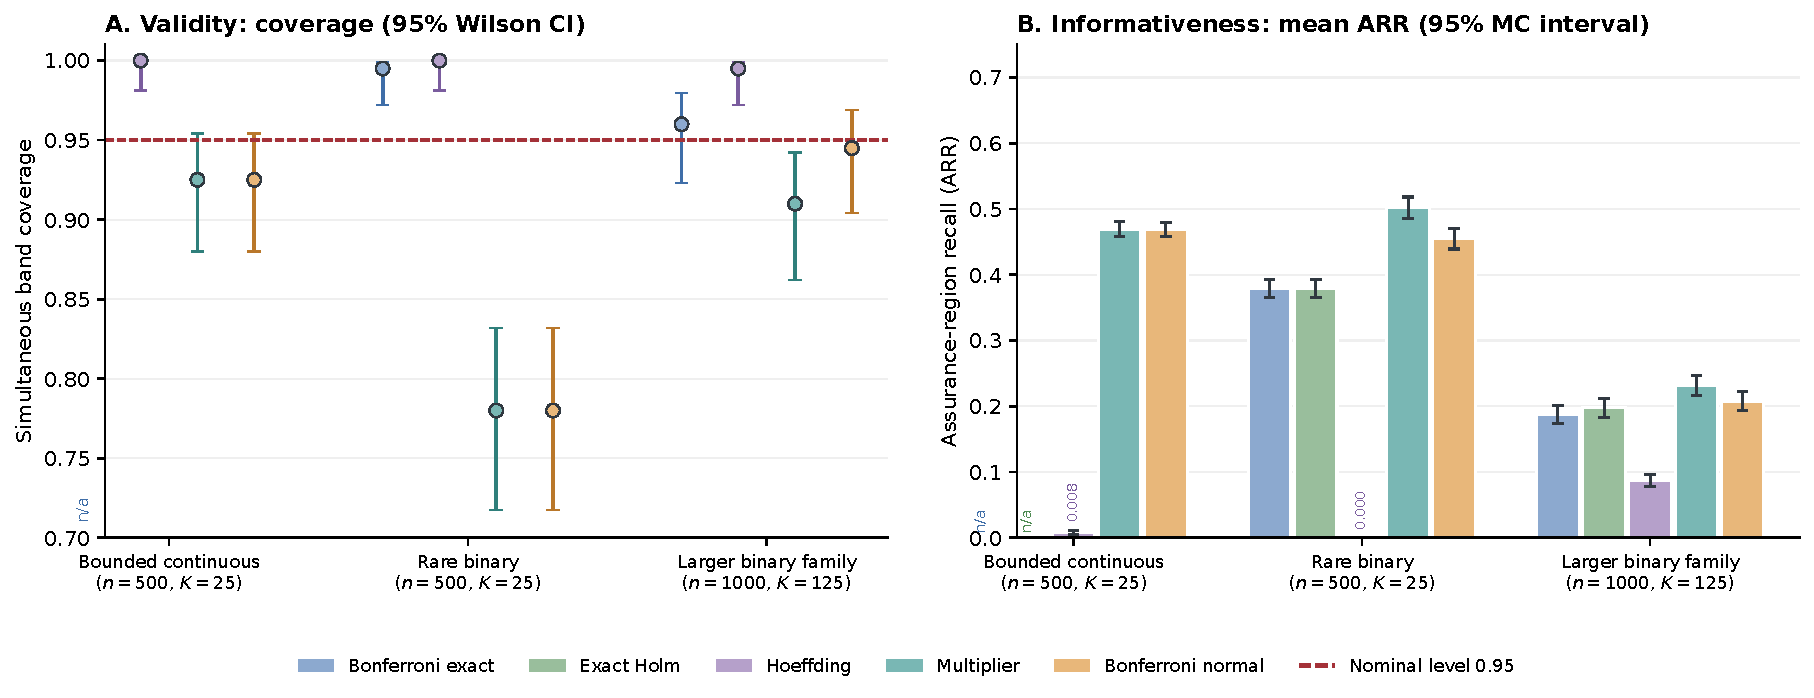
\includegraphics[width=\linewidth]{stress_validity.pdf}
\caption{Adverse regimes (\StressReps{} replications per design). (A) Simultaneous band
coverage with 95\% Wilson intervals; the dashed line is the nominal level. (B) Mean ARR with
95\% Monte Carlo intervals. ``n/a'' marks procedures that do not apply: exact binomial bounds
for continuous losses and, in panel A, exact Holm, which has no band. Bonferroni normal and the
multiplier have identical coverage in the first two designs, as explained in
Section~\ref{sec:calibration}.}
\label{fig:stress}
\end{figure}

\begin{figure}[ht]
\centering\includegraphics[width=.96\linewidth]{sensitivity.pdf}
\caption{Coverage and recall sensitivity to the assurance sample size and dependence. Latent
Gaussian correlation is a generator parameter, not the observed binary-loss correlation. Holm
is omitted from the coverage panels.}
\label{fig:sensitivity}
\end{figure}

\begin{table}[ht]
\centering\small
\caption{Paired mean ARR gain of the multiplier over each comparator in the sensitivity study.
MCSE uses paired replication differences. These efficiency comparisons must be read together
with the coverage results.}
\label{tab:gains}\begin{tabular}{rrlrr}
\toprule
$n$ & $\rho$ & Comparator & Paired ARR gain & MCSE \\
\midrule
500 & 0.55 & Bonferroni normal & 0.009 & 0.0016 \\
1000 & 0.10 & Bonferroni normal & -0.000 & 0.0008 \\
1000 & 0.55 & Bonferroni normal & 0.012 & 0.0016 \\
1000 & 0.90 & Bonferroni normal & 0.066 & 0.0038 \\
5000 & 0.55 & Bonferroni normal & 0.012 & 0.0017 \\
500 & 0.55 & Bonferroni exact & 0.037 & 0.0029 \\
1000 & 0.10 & Bonferroni exact & 0.020 & 0.0020 \\
1000 & 0.55 & Bonferroni exact & 0.036 & 0.0029 \\
1000 & 0.90 & Bonferroni exact & 0.092 & 0.0041 \\
5000 & 0.55 & Bonferroni exact & 0.016 & 0.0019 \\
500 & 0.55 & Exact Holm & 0.035 & 0.0029 \\
1000 & 0.10 & Exact Holm & 0.011 & 0.0016 \\
1000 & 0.55 & Exact Holm & 0.024 & 0.0023 \\
1000 & 0.90 & Exact Holm & 0.080 & 0.0041 \\
5000 & 0.55 & Exact Holm & 0.003 & 0.0010 \\
\bottomrule
\end{tabular}

\end{table}
\begin{table}[ht]
\centering\small\setlength{\tabcolsep}{4pt}
\caption{Validity in the power study of Section~\ref{sec:power}: minimum band coverage over the
24 cells of each family size, the minimum at $n=250$, minimum containment at $\tau=.10$, and
maximum UCP. Exact Holm supplies fixed-tolerance tests and has no band.}
\label{tab:power-validity}\begin{tabular}{lrrrrr}
\toprule
 & & \multicolumn{2}{c}{Band coverage (min.)} & Containment & UCP \\
\cmidrule(lr){3-4}
Method & $K$ & all $n$ & $n=250$ & (min.) & (max.) \\
\midrule
Bonferroni exact & 25 & 0.948 & 0.983 & 1.000 & 0.0000 \\
Bonferroni exact & 100 & 0.948 & 0.975 & 0.998 & 0.0008 \\
Exact Holm & 25 & -- & -- & 1.000 & 0.0000 \\
Exact Holm & 100 & -- & -- & 0.998 & 0.0008 \\
Hoeffding & 25 & 1.000 & 1.000 & 1.000 & 0.0000 \\
Hoeffding & 100 & 1.000 & 1.000 & 1.000 & 0.0000 \\
Multiplier & 25 & 0.810 & 0.810 & 0.983 & 0.0096 \\
Multiplier & 100 & 0.610 & 0.610 & 0.965 & 0.0126 \\
\bottomrule
\end{tabular}

\end{table}
\begin{table}[ht]
\centering\small\setlength{\tabcolsep}{4pt}
\caption{Exact one-sided failure probability of the studentized normal upper bound
$\widehat R_k+z_{1-\alpha/K}\widehat\sigma_k/\sqrt n$ for one environment with risk $R_k$, as a
multiple of its nominal value $\alpha/K$ ($\alpha=.05$). Values are computed from the binomial
distribution without simulation; a value of 1 would indicate exact calibration.}
\label{tab:tail}\begin{tabular}{rrrrrrrrr}
\toprule
$K$ & $R_k$ & $n=250$ & $n=500$ & $n=1,000$ & $n=2,000$ & $n=4,000$ & $n=8,000$ & $n=32,000$ \\
\midrule
25 & 0.05 & 6.54 & 5.41 & 2.96 & 2.29 & 1.63 & 1.52 & 1.24 \\
25 & 0.09 & 4.55 & 2.71 & 2.50 & 1.81 & 1.59 & 1.31 & 1.19 \\
25 & 0.11 & 4.65 & 2.22 & 1.95 & 1.52 & 1.50 & 1.27 & 1.16 \\
25 & 0.15 & 3.98 & 1.94 & 1.84 & 1.38 & 1.26 & 1.17 & 1.13 \\
100 & 0.05 & 26.17 & 11.02 & 4.39 & 3.23 & 2.45 & 1.80 & 1.36 \\
100 & 0.09 & 8.60 & 6.42 & 3.29 & 2.53 & 1.72 & 1.61 & 1.20 \\
100 & 0.11 & 9.60 & 3.29 & 2.79 & 2.32 & 1.83 & 1.53 & 1.24 \\
100 & 0.15 & 4.90 & 3.31 & 2.23 & 1.92 & 1.53 & 1.31 & 1.15 \\
500 & 0.05 & 45.71 & 26.10 & 7.19 & 5.06 & 3.12 & 2.33 & 1.60 \\
500 & 0.09 & 18.63 & 10.10 & 4.70 & 2.90 & 2.47 & 1.85 & 1.38 \\
500 & 0.11 & 10.47 & 9.61 & 4.46 & 3.06 & 2.01 & 1.75 & 1.33 \\
500 & 0.15 & 12.69 & 6.52 & 2.92 & 2.34 & 1.70 & 1.60 & 1.25 \\
\bottomrule
\end{tabular}

\end{table}
\begin{table}[ht]
\centering\small
\caption{Equally spaced WDBC logistic-regression grids.}
\label{tab:grid}\begin{tabular}{llrrr}
\toprule
Grid & Method & $K$ & Certified $\tau=.08$ & Fraction \\
\midrule
$4\times4$ & Multiplier & 16 & 10 & 0.625 \\
$4\times4$ & Bonferroni exact & 16 & 7 & 0.438 \\
$6\times6$ & Multiplier & 36 & 23 & 0.639 \\
$6\times6$ & Bonferroni exact & 36 & 11 & 0.306 \\
$10\times10$ & Multiplier & 100 & 69 & 0.690 \\
$10\times10$ & Bonferroni exact & 100 & 23 & 0.230 \\
\bottomrule
\end{tabular}

\end{table}
\FloatBarrier

\section{Continuous Example and Independent Pilot}
\label{app:continuous}
The illustrative surface $R(m,s)=.24+.12m+.10s+.05ms$ on $[0,.4]\times[0,.6]$ has the valid
Euclidean Lipschitz bound $L_R=\sqrt{.15^2+.12^2}$. We use a $5\times5$ assurance grid,
$\tau=.32$, \ContReps{} replications, and an $81\times81$ mesh for numerical recall and
containment diagnostics. The analytical argument for \eqref{eq:continuous}, not the mesh,
supplies coverage at every point when the grid band and the global bound are valid; the mesh
values approximate geometric behavior only (Table~\ref{tab:continuous}). Separate exports
evaluate half and twice the analytic bound; the half bound is not asserted to be valid.

In the first replication (Figure~\ref{fig:continuous}A), fixed in advance rather than
selected, exact Bonferroni certified \ContExactFirstGrid{} of the \ContExactFirstSafeGrid{}
acceptable grid points, the Lipschitz extension certified \ContExactFirstRecall{} of the
acceptable mesh area (the multiplier certified \ContMultFirstRecall), and
\ifnum\ContExactFirstUnsafe=0 no unacceptable mesh point was certified\else\ContExactFirstUnsafe{} unacceptable mesh points were certified\fi. The extension is
conservative near the boundary because the term $L_R\dist(e,e_k)$ is added to bounds that
already carry the multiplicity correction.

The pilot example starts with an $11\times11$ candidate grid on the same rectangle. Using 300
independent pilot rows, it retains points whose pilot risks are within $.015$ of $.32$ together
with the coordinate extremes, and then certifies the selected family on new assurance rows
with exact Bonferroni over 200 replications. This demonstrates a valid split-sample design; it
does not establish an optimal adaptive grid or certification of unselected points.

\begin{table}[ht]
\centering\small
\caption{Continuous example over \ContReps{} replications. Grid coverage is band coverage on the
$5\times5$ grid; mesh containment and recall are evaluated on an $81\times81$ mesh, where recall
is an equal-grid-point area approximation.}
\label{tab:continuous}\begin{tabular}{lrrrr}
\toprule
Method & Grid coverage & Mesh containment & Mesh recall & Mesh UCP \\
\midrule
Bonferroni exact & 0.965 & 0.980 & 0.404 & 0.0001 \\
Hoeffding & 1.000 & 1.000 & 0.185 & 0.0000 \\
Multiplier & 0.940 & 0.975 & 0.460 & 0.0004 \\
\bottomrule
\end{tabular}

\end{table}
\begin{figure}[ht]
\centering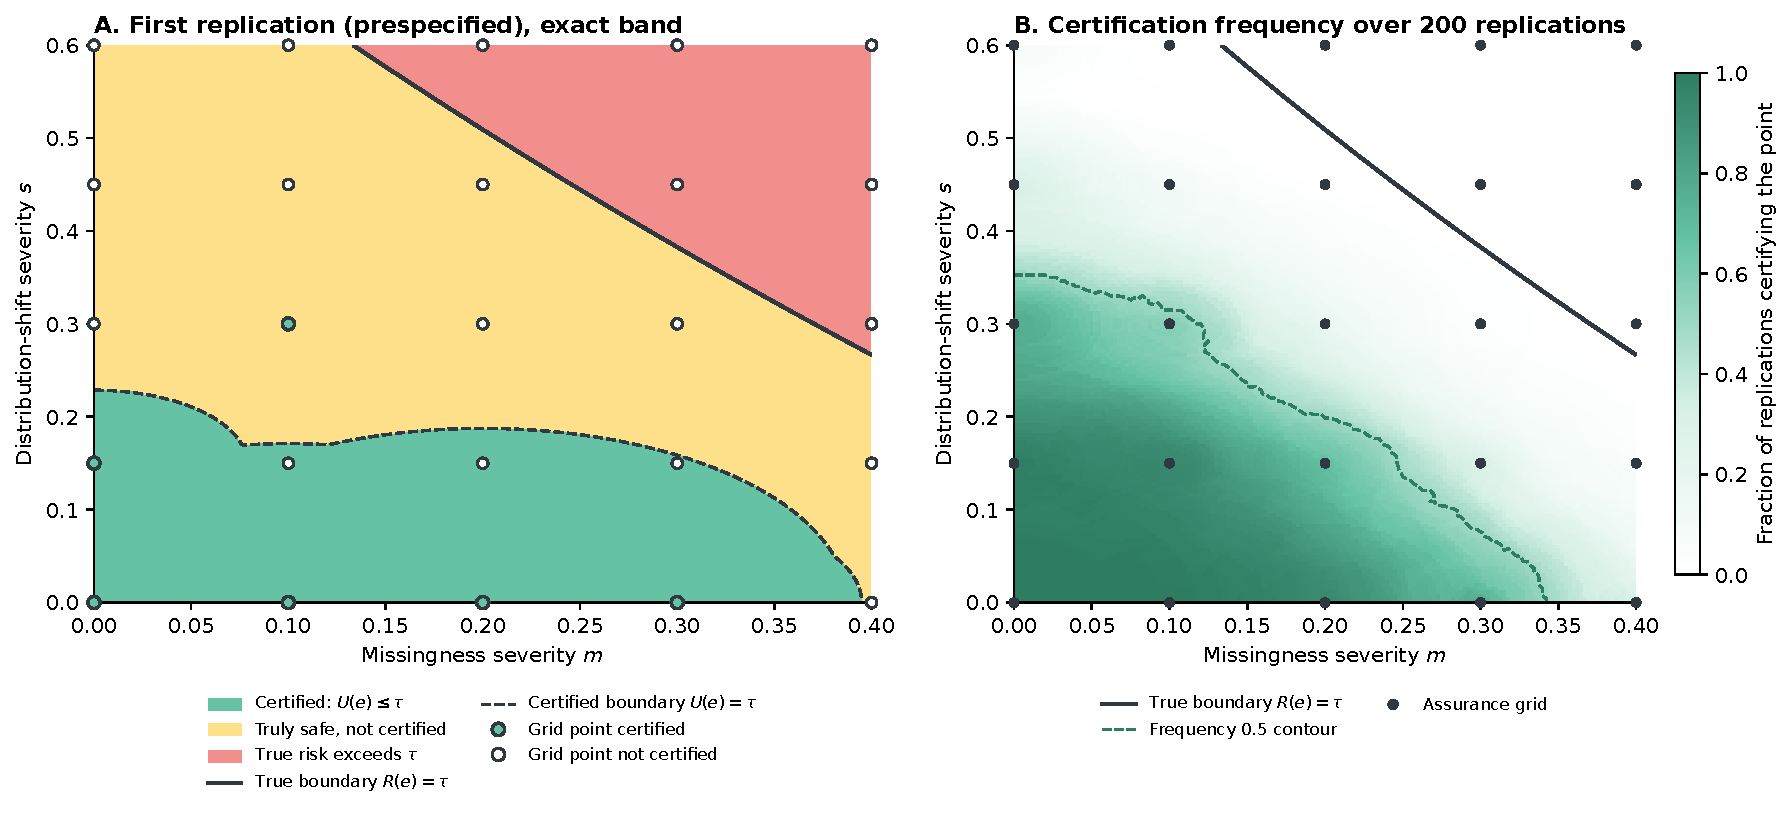
\includegraphics[width=\linewidth]{continuous_exact.pdf}
\caption{Continuous example with the exact Clopper--Pearson Bonferroni grid band and the
Lipschitz extension \eqref{eq:continuous} ($5\times5$ grid, $\tau=.32$). (A) The first of the
\ContReps{} replications: green is the certified region, yellow is acceptable but not
certified, and red has true risk above $\tau$; filled green markers are certified grid points.
The certified point at $(m,s)=(0.1,0.3)$ has an upper bound just below $\tau$, so its
certified neighborhood is smaller than its marker. (B) Fraction of replications in which each
point is certified, with the 0.5 contour.}
\label{fig:continuous}
\end{figure}
\FloatBarrier

\section{Computational Cost and Bootstrap Variability}
\label{app:runtime}
The direct multiplier sampler requires $O(BnK)$ operations. Sampling from its conditional
Gaussian covariance instead costs $O(nK^2+K^3+BK^2)$ and stores a $K\times K$ matrix, which can
be advantageous for moderate $K$; the code uses it when $K\leq\min(n,2000)$ and otherwise uses
a chunked row-multiplier sampler. Conditional distributional equivalence of the two samplers is
tested with identical-column and independent-column constructions; numerical agreement between
samplers does not verify frequentist coverage. The timing study holds the loss matrix fixed and
repeats each bootstrap size under 25 independent seeds (Table~\ref{tab:runtime}). Timings depend
on the machine and numerical libraries and exclude loss generation and model fitting. The
critical-value MCSE is the standard error of its mean across seeds, not a guaranteed quantile
error bound.
\begin{table}[ht]
\centering\small
\caption{Conditional-covariance multiplier timing and variability.}
\label{tab:runtime}\begin{tabular}{lrrrrr}
\toprule
$n$ & $K$ & $B$ & Critical mean & Critical MCSE & Mean seconds \\
\midrule
500 & 25 & 200 & 2.819 & 0.0188 & 0.0019 \\
500 & 25 & 1000 & 2.795 & 0.0085 & 0.0022 \\
500 & 25 & 5000 & 2.796 & 0.0052 & 0.0057 \\
1000 & 25 & 200 & 2.806 & 0.0289 & 0.0018 \\
1000 & 25 & 1000 & 2.793 & 0.0089 & 0.0028 \\
1000 & 25 & 5000 & 2.794 & 0.0037 & 0.0077 \\
1000 & 125 & 200 & 3.257 & 0.0227 & 0.0104 \\
1000 & 125 & 1000 & 3.213 & 0.0097 & 0.0127 \\
1000 & 125 & 5000 & 3.210 & 0.0035 & 0.0413 \\
\bottomrule
\end{tabular}

\end{table}

\section{High-Dimensional Gaussian Approximation}
\label{app:highdim}
For increasing $K$, the Gaussian-approximation results of \citet{chernozhukov2013gaussian}
provide sufficient regimes for bounded coordinates with uniformly positive variances; a familiar
conservative regime is $\log^7(Kn)/n\to0$ under the associated regularity constants.
Lemma~\ref{lem:rows} establishes the independent-vector construction, and bounded losses with a
uniform variance lower bound supply the basic moment conditions. Later refinements improve
Gaussian and bootstrap approximation rates \citep{cckk2022}. We do not assert their sharpest
rates for the present grouped and stressed-data implementation, and none of them is used as a
practical sample-size prescription; the finite-sample experiments assess the approximation
directly.

\section{Planning Table, Verification, and Reproduction}
\label{app:verification}
Table~\ref{tab:planning} gives assurance sample sizes sufficient for a Hoeffding additive width
of at most the stated margin; Table~\ref{tab:power-planning} gives the exact alternative based on
certification probability.
\begin{table}[ht]
\centering\small
\caption{Conservative assurance-sample planning for a Hoeffding additive width at most the
stated margin, with $\alpha=.05$. This is not a guarantee of a particular recall.}
\label{tab:planning}\begin{tabular}{lrr}
\toprule
$K$ & Margin & Sufficient $n$ \\
\midrule
25 & 0.02 & 7769 \\
25 & 0.05 & 1243 \\
25 & 0.10 & 311 \\
100 & 0.02 & 9502 \\
100 & 0.05 & 1521 \\
100 & 0.10 & 381 \\
500 & 0.02 & 11513 \\
500 & 0.05 & 1843 \\
500 & 0.10 & 461 \\
\bottomrule
\end{tabular}

\end{table}

The test suite checks the finite-sample binomial error by enumerating possible counts, the
zero-error bound, empirical degeneracy, duplicated columns, the equivalence of the covariance
and row multiplier samplers, unequal samples, overlapping and empty groups, reference
boundaries, MAR row locality, ATC ties, and the admission-aligned MIMIC-IV cohort
construction. Further tests check the exact certification threshold of \eqref{eq:pcert}
against brute-force enumeration of Clopper--Pearson bounds, the closed-form certification
probability, the zero-false-negative bound and minimum death count of Section~\ref{sec:mimic},
the planning search, and the monotonicity of the tolerance--certification profiles. The
aggregate-output schema is also exercised on a synthetic data set with the structure of the
MIMIC-IV tables, which is used only for testing. The notebook imports the same functions,
records configuration and package versions, and generates all manuscript inputs from completed
runs; no reported result was selected by changing the seed.

The original full run used Python \OrigPython{} with NumPy \OrigNumpy, and the supplementary
analyses used Python \RevPython{} with NumPy \RevNumpy, SciPy \RevScipy, pandas \RevPandas, and
scikit-learn \RevSklearn. Regenerating the primary calibration from its archived seeds in the
newer environment reproduced all \AnatReps{} replications exactly for exact Bonferroni, exact
Holm, Hoeffding, Bonferroni normal, and pointwise normal (Table~\ref{tab:anatomy}). The
multiplier reproduced \AnatMultReproduced{} of \AnatReps{} replications, and its regenerated
coverage was \AnatMultCoverageRerun{} rather than \CalMultCoverage. This difference does not
reflect a change in the method: the multiplier critical value depends on Gaussian draws produced
through an eigendecomposition whose output, for example eigenvector signs, can differ across
numerical libraries, so the same seed yields different but identically distributed draws. For
the fixed loss matrices of the timing study, the regenerated critical values differed from the
archived ones with standard deviation \BootDiffSdLow{} at $B=\BootDiffBLow$ and \BootDiffSdHigh{}
at $B=\BootDiffBHigh$, the scale of Monte Carlo error. Bitwise reproduction of multiplier
decisions requires archiving the critical value or the draws, and all multiplier results in the
main text are those of the original archived run.
\begin{table}[ht]
\centering\small\setlength{\tabcolsep}{4pt}
\caption{Decomposition of band failures in the regenerated primary calibration (\AnatReps{}
replications, $\tau=.34$). ``Reproduced'' counts replications whose coverage, certified count,
and ARR match the archived run. Band failures are split into those that missed only acceptable
environments and those that missed at least one unacceptable environment. Containment failures
are replications that certified an unacceptable environment at $\tau=.34$.}
\label{tab:anatomy}\begin{tabular}{lrrrrr}
\toprule
 & & Band & \multicolumn{2}{c}{Failures that missed} & Containment \\
\cmidrule(lr){4-5}
Method & Reproduced & failures & only acceptable & an unacceptable & failures \\
\midrule
Bonferroni exact & 500/500 & 20 & 9 & 11 & 1 \\
Exact Holm & 500/500 & -- & -- & -- & 1 \\
Hoeffding & 500/500 & 0 & 0 & 0 & 0 \\
Multiplier & 466/500 & 34 & 19 & 15 & 1 \\
Bonferroni normal & 500/500 & 31 & 18 & 13 & 1 \\
Pointwise normal & 500/500 & 243 & 89 & 154 & 21 \\
\bottomrule
\end{tabular}

\end{table}
\FloatBarrier

\section{Provenance of Reported Results}
\label{app:provenance}
The base seed is $s=20260927$, and $S(a,\ldots)$ denotes the integer seed returned by NumPy's
\texttt{SeedSequence} with inputs $(s,a,\ldots)$, where $r$ indexes replications and $j$
indexes settings. The primary script \texttt{scripts/run\_analysis.py} produced, from archived
outputs, the primary calibration (losses $S(10,r)$, multiplier $S(11,r)$), the adverse regimes
($S(32,j,r)$, $S(33,j,r)$), the sensitivity study and paired gains ($S(20,j,r)$, $S(21,j,r)$),
the independent pilot ($S(80,r)$, $S(81,r)$), the nested refits and ATC predictions
($S(40,r)$--$S(44,r)$, multiplier $S(45,r)$), the missingness study ($S(50,r)$--$S(53,r)$,
multiplier $S(54,r)$), the WDBC analyses (split and model seed 42, perturbations $s$,
multiplier $S(60)$), the runtime study ($S(30,n,K)$, $S(31,r)$), and the Hoeffding planning
table. The MIMIC-IV misclassification analysis was produced by \texttt{scripts/run\_mimic.py}
or the equivalent notebook call (split, models, and missingness $s$; multiplier $s+1$), the
false-negative analysis by the notebook (multiplier $s+8001$), and the operating
characteristics by the notebook function \texttt{mimic\_class\_sensitive\_operating}, which
reuses $s$ without additional bootstrap draws and was checked against the saved thresholds and
false-negative counts.

The supplementary script \texttt{scripts/run\_revision.py} produced the power study (new
simulations with seeds $S(90,i_K,i_n,i_\Delta,r)$ and $S(91,i_K,i_n,i_\Delta,r)$), the exact
continuous bounds (reusing the losses $S(70,r)$), the decomposition of calibration failures and
the adverse-regime critical values (regenerated from the original seeds), and the bootstrap
reproduction diagnostics. The exact planning table, the tail calculation, the
tolerance--certification profiles, and the MIMIC-IV effective-sample-size summaries are
deterministic calculations from saved outputs. Here ``archived'' means that values come from
saved outputs of the original run even when a display was rendered again, ``regenerated''
means that the analysis was executed again, and reused seeds identify the original
random-number construction rather than guaranteeing identical floating-point results across
computing environments.

\end{document}
